\documentclass[10pt,a4paper]{article}

\usepackage[T1]{fontenc}
\usepackage[utf8]{inputenc}
\usepackage{lmodern}
\usepackage[margin=1.75cm,top=1.7cm,bottom=1.7cm]{geometry}
\usepackage{microtype}
\DisableLigatures{encoding = *, family = tt*}
\usepackage{booktabs}
\usepackage{tabularx}
\usepackage{longtable}
\usepackage{array}
\usepackage{enumitem}
\usepackage{amsmath,amssymb}
\usepackage{float}
\usepackage{caption}
\usepackage{fancyhdr}
\usepackage{tikz}
\usepackage{xcolor}
\usepackage[obeyspaces,spaces]{url}
\usepackage[hidelinks]{hyperref}

\usetikzlibrary{arrows.meta,positioning,shapes.geometric,fit,calc,backgrounds}

\setlength{\parindent}{0pt}
\setlength{\parskip}{0.31em}
\setlength{\emergencystretch}{1.8em}
\setlist{itemsep=0.10em,topsep=0.18em,parsep=0.05em,leftmargin=1.4em}
\renewcommand{\arraystretch}{1.13}
\captionsetup{font=small,labelfont=bf,skip=4pt}

% Compact headings: no huge chapter pages or oversized titles
\usepackage{titlesec}
\titleformat{\section}{\large\bfseries\color{black!90}}{\thesection}{0.6em}{}[\vspace{-0.3em}\rule{\textwidth}{0.4pt}]
\titleformat{\subsection}{\normalsize\bfseries\color{black!85}}{\thesubsection}{0.5em}{}
\titleformat{\subsubsection}{\small\bfseries\color{black!80}}{\thesubsubsection}{0.4em}{}
\titlespacing*{\section}{0pt}{0.9em}{0.35em}
\titlespacing*{\subsection}{0pt}{0.65em}{0.25em}
\titlespacing*{\subsubsection}{0pt}{0.45em}{0.15em}

\pagestyle{fancy}
\fancyhf{}
\fancyhead[L]{\footnotesize MP-QUIC Mini: Technical Documentation Report}
\fancyhead[R]{\footnotesize Implementation Reference}
\fancyfoot[C]{\footnotesize\thepage}
\renewcommand{\headrulewidth}{0.3pt}

\newcommand{\codeul}{\textunderscore\hspace{0pt}}
\DeclareRobustCommand{\code}[1]{{\ttfamily\let\_\codeul #1}}
\newcolumntype{L}[1]{>{\raggedright\arraybackslash}p{#1}}
\newcolumntype{Y}{>{\raggedright\arraybackslash}X}

\begin{document}

% Start directly with title and introduction (no cover page, no TOC)
\begin{center}
    {\Large\bfseries MP-QUIC Mini: Complete Technical Documentation Report}\\[0.25em]
    {\small\textit{Architecture, Wire Format, Reliability, Coupled Congestion Control, Linux I/O, and Multi-VM Deployment of the Implemented C++17 Protocol}}
\end{center}
\vspace{0.2em}
\hrule
\vspace{0.5em}

% ==============================================================================
\section{Introduction and Problem Statement}
% ==============================================================================

\subsection{Motivation and Problem Statement}
Modern networked devices—such as smartphones with Wi-Fi and LTE/5G radios, laptops with Ethernet and wireless adapters, and multi-homed servers—routinely possess multiple network interfaces. Standard transport protocols, however, bind a connection to a single static 4-tuple $(\text{source IP}, \text{source port}, \text{destination IP}, \text{destination port})$. This single-path binding creates two fundamental limitations: (1) an application cannot aggregate the bandwidth of multiple available links within one transport session, and (2) when the active interface fails or degrades (for example, a user walking out of Wi-Fi range), the transport session stalls or breaks, forcing upper layers to open a new connection.

\textbf{MP-QUIC Mini} is a modular, user-space C++17 implementation of Multipath QUIC inspired by the design of De Coninck and Bonaventure (ACM CoNEXT 2017). It implements a reliable, flow-controlled, congestion-controlled, and multipath-capable transport protocol directly over Linux UDP sockets without requiring kernel modifications.

\subsection{Why UDP Alone Is Insufficient and Single-Path Limits}
Standard User Datagram Protocol (UDP) provides only a thin, connectionless datagram service over IPv4/IPv6 with port multiplexing and an optional checksum. UDP offers:
\begin{itemize}
    \item \textbf{No reliability:} Datagrams may be silently dropped, duplicated, or reordered by intermediate routers.
    \item \textbf{No byte-stream abstraction:} Applications receive discrete datagrams rather than an ordered, contiguous byte stream.
    \item \textbf{No flow control:} A fast sender can overwhelm a slow receiver's buffers.
    \item \textbf{No congestion control:} Unchecked UDP traffic can saturate network queues and starve competing TCP flows.
    \item \textbf{No connection identity:} There is no protocol-level session identifier independent of IP/port tuples.
\end{itemize}

Conversely, standard TCP provides reliability, ordering, flow control, and congestion control, but suffers from three structural drawbacks for multipath evolution: (i) TCP resides in the OS kernel, slowing deployment; (ii) TCP ties reliability and ordering to a single contiguous sequence-number space bound to one 4-tuple; and (iii) Multipath TCP (MPTCP) requires kernel support and faces middlebox interference when TCP options are stripped or rewritten.

\subsection{Multipath Communication, MP-QUIC, and MP-QUIC Mini}
Multipath communication decouples the logical transport connection from individual network paths. By running in user space atop UDP, QUIC avoids middlebox ossification of TCP headers and allows rapid iteration. Multipath QUIC (MP-QUIC) extends QUIC so that a single connection—identified by a 64-bit Connection ID—can simultaneously transmit and receive packets across multiple network paths, each identified by a Path ID.

\textbf{MP-QUIC Mini} implements the core transport mechanics of the CoNEXT 2017 MP-QUIC architecture in approximately 3,200 lines of library C++17 code, accompanied by end-to-end file transfer and latency-benchmarking tools (\code{mpq\_server}, \code{mpq\_client}, \code{mpq\_reqres}) and a 10-suite test harness.

\subsection{Concepts Borrowed from QUIC vs.\ Differences from Standard QUIC}
Table~\ref{tab:quic_diff} contrasts the QUIC/MP-QUIC concepts retained in MP-QUIC Mini against features of standard IETF QUIC (RFC 9000) and the full CoNEXT 2017 Go reference implementation that are simplified or omitted.

\begin{table}[H]
\centering
\footnotesize
\begin{tabularx}{\textwidth}{p{3.6cm}p{5.8cm}X}
\toprule
\textbf{Protocol Aspect} & \textbf{Adopted in MP-QUIC Mini} & \textbf{Difference from Standard QUIC / Full MP-QUIC} \\
\midrule
Connection Identity & 64-bit \code{connection\_id} in every packet header; survives NAT rebinding. & Single fixed 8-byte ID per connection; no variable-length CIDs or CID rotation. \\
Framing & Self-delimiting frames (\code{STREAM}, \code{ACK}, \code{WINDOW\_UPDATE}, \code{PING}, \code{ADD\_ADDRESS}, \code{PATHS}, \code{CONNECTION\_CLOSE}). & Fixed-width fields in headers; only ACK ranges use 2-bit-prefixed varints. \code{CLOSE\_PATH} (\code{0x11}) is reserved, not implemented. \\
Per-Path Number Space & Independent 64-bit \code{packet\_number} per \code{path\_id} starting at 1; \code{ACK} includes \code{path\_id}. & No packet-number encryption/truncation; full 64-bit number transmitted in plaintext. \\
Security \& Handshake & None (explicitly omitted). & No TLS 1.3 handshake, no AEAD payload encryption, no header protection, no retry/stateless reset. \\
Path Management & \code{ADD\_ADDRESS} frame from server; client opens odd \code{path\_id}s; \code{PING} probes new paths. & No \code{CLOSE\_PATH}; server passively creates paths on first valid packet; fixed initial flow-control windows. \\
Congestion Control & Per-path \code{OliaSender} (coupled OLIA) + \code{HybridSlowStart}. & OLIA halves \code{cwnd} on loss (\code{OLIA\_LOSS\_WINDOW\_DIVISOR = 2}) rather than CUBIC's $0.85$ factor noted in code comments. \\
Loss Recovery & Time-based loss ($9/8\times\text{RTT}$), 2 TLPs, exponential RTO, \code{potentially\_failed} marking. & No packet-threshold (e.g., 3-packet) loss detection; no packet pacing. \\
\bottomrule
\end{tabularx}
\caption{Comparison between MP-QUIC Mini and standard QUIC / full CoNEXT 2017 MP-QUIC.}
\label{tab:quic_diff}
\end{table}

\subsection{Project Objectives and Expected Benefits}
The project aims to: (1) construct a modular user-space multipath transport engine over Linux \code{epoll} and non-blocking UDP sockets; (2) guarantee strict in-order, exactly-once byte-stream delivery despite cross-path reordering and packet loss; (3) aggregate throughput across heterogeneous paths while maintaining TCP fairness via OLIA; and (4) survive mid-transfer link failures via path-failure detection, \code{PATHS} signaling, and cross-path retransmission.

% ==============================================================================
\section{Overall Architecture}
% ==============================================================================

\subsection{End-to-End Sender and Receiver Architecture}
MP-QUIC Mini is organized as an event-driven, single-threaded reactor per endpoint. Every application (\code{mpq\_server}, \code{mpq\_client}, \code{mpq\_reqres}) instantiates a \code{SocketManager} that monitors one or more \code{UDPSocket} file descriptors via Linux \code{epoll} and drives protocol timers via periodic \code{on\_tick()} callbacks. Figure~\ref{fig:arch} illustrates the complete sender-side and receiver-side module architecture and data/control flows as implemented in the repository.

\begin{figure}[H]
\centering
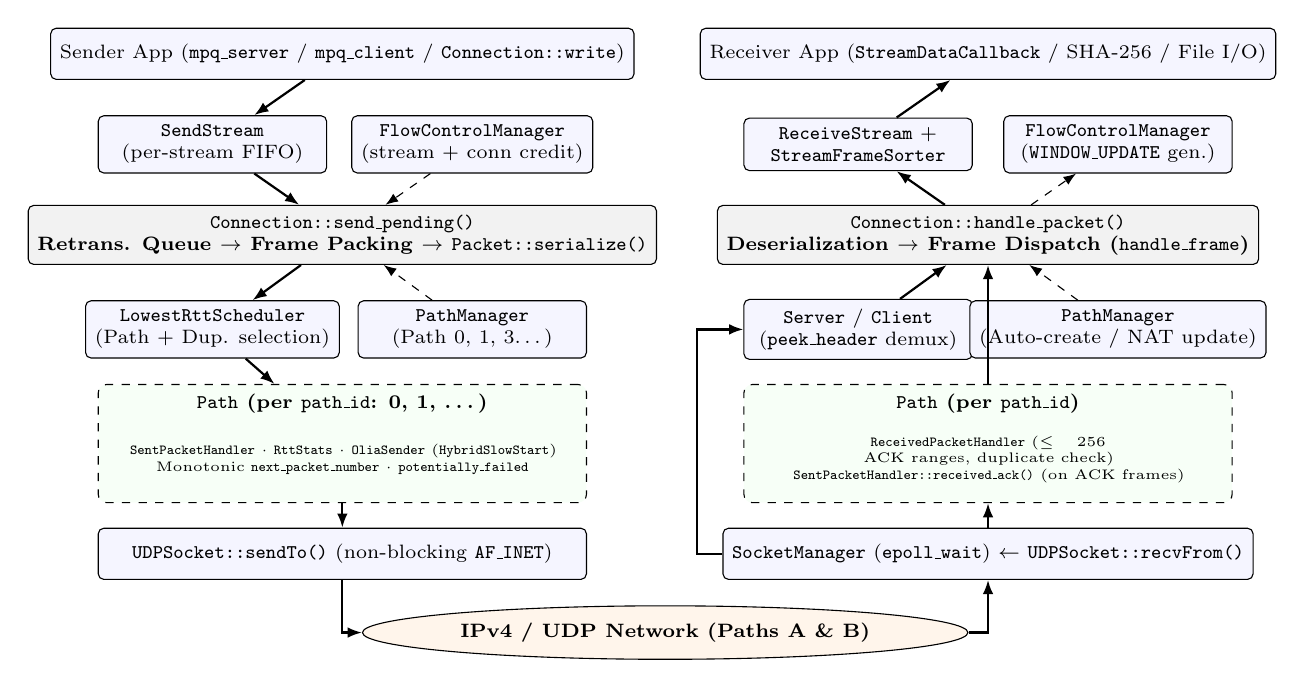
\begin{tikzpicture}[
    mod/.style={draw, rectangle, rounded corners=2pt, minimum height=0.65cm, align=center, font=\scriptsize, fill=blue!4},
    core/.style={draw, rectangle, rounded corners=2pt, minimum height=0.75cm, align=center, font=\scriptsize\bfseries, fill=gray!10},
    pathbox/.style={draw, dashed, rectangle, rounded corners=3pt, inner sep=4pt, fill=green!3},
    arr/.style={-{Latex[length=1.8mm]}, thick},
    darr/.style={-{Latex[length=1.6mm]}, dashed}
]
% Sender side (Left, x = 0)
\node[mod, minimum width=6.2cm] (sapp) at (0, 6.3) {Sender App (\code{mpq\_server} / \code{mpq\_client} / \code{Connection::write})};
\node[mod, minimum width=2.9cm] (sstream) at (-1.65, 5.15) {\code{SendStream}\\(per-stream FIFO)};
\node[mod, minimum width=2.9cm] (sfc) at (1.65, 5.15) {\code{FlowControlManager}\\(stream + conn credit)};
\node[core, minimum width=6.2cm] (sconn) at (0, 4.0) {\code{Connection::send\_pending()}\\Retrans. Queue $\rightarrow$ Frame Packing $\rightarrow$ \code{Packet::serialize()}};
\node[mod, minimum width=2.9cm] (ssched) at (-1.65, 2.8) {\code{LowestRttScheduler}\\(Path + Dup. selection)};
\node[mod, minimum width=2.9cm] (spmgr) at (1.65, 2.8) {\code{PathManager}\\(Path 0, 1, 3\dots)};

\node[pathbox, minimum width=6.2cm, minimum height=1.5cm] (spath) at (0, 1.35) {};
\node[font=\scriptsize\bfseries, anchor=north] at (spath.north) {\code{Path} (per \code{path\_id}: 0, 1, \dots)};
\node[font=\tiny, align=center, text width=5.9cm] at (0, 1.15) {\code{SentPacketHandler} $\cdot$ \code{RttStats} $\cdot$ \code{OliaSender} (\code{HybridSlowStart})\\Monotonic \code{next\_packet\_number} $\cdot$ \code{potentially\_failed}};

\node[mod, minimum width=6.2cm] (ssock) at (0, -0.05) {\code{UDPSocket::sendTo()} (non-blocking \code{AF\_INET})};

% Receiver side (Right, x = 8.2)
\node[mod, minimum width=6.2cm] (rapp) at (8.2, 6.3) {Receiver App (\code{StreamDataCallback} / SHA-256 / File I/O)};
\node[mod, minimum width=2.9cm] (rstream) at (6.55, 5.15) {\code{ReceiveStream} +\\ \code{StreamFrameSorter}};
\node[mod, minimum width=2.9cm] (rfc) at (9.85, 5.15) {\code{FlowControlManager}\\(\code{WINDOW\_UPDATE} gen.)};
\node[core, minimum width=6.2cm] (rconn) at (8.2, 4.0) {\code{Connection::handle\_packet()}\\Deserialization $\rightarrow$ Frame Dispatch (\code{handle\_frame})};
\node[mod, minimum width=2.9cm] (rendp) at (6.55, 2.8) {\code{Server} / \code{Client}\\(\code{peek\_header} demux)};
\node[mod, minimum width=2.9cm] (rpmgr) at (9.85, 2.8) {\code{PathManager}\\(Auto-create / NAT update)};

\node[pathbox, minimum width=6.2cm, minimum height=1.5cm] (rpath) at (8.2, 1.35) {};
\node[font=\scriptsize\bfseries, anchor=north] at (rpath.north) {\code{Path} (per \code{path\_id})};
\node[font=\tiny, align=center, text width=5.9cm] at (8.2, 1.15) {\code{ReceivedPacketHandler} ($\le 256$ ACK ranges, duplicate check)\\\code{SentPacketHandler::received\_ack()} (on ACK frames)};

\node[mod, minimum width=6.2cm] (rsock) at (8.2, -0.05) {\code{SocketManager} (\code{epoll\_wait}) $\leftarrow$ \code{UDPSocket::recvFrom()}};

% Network cloud
\node[draw, ellipse, minimum width=3.6cm, minimum height=0.65cm, font=\scriptsize\bfseries, fill=orange!8] (net) at (4.1, -1.05) {IPv4 / UDP Network (Paths A \& B)};

% Sender arrows
\draw[arr] (sapp) -- (sstream);
\draw[arr] (sstream) -- (sconn);
\draw[darr] (sfc) -- (sconn);
\draw[arr] (sconn) -- (ssched);
\draw[darr] (spmgr) -- (sconn);
\draw[arr] (ssched) -- (spath);
\draw[arr] (spath) -- (ssock);
\draw[arr] (ssock.south) |- (net.west);

% Receiver arrows
\draw[arr] (net.east) -| (rsock.south);
\draw[arr] (rsock.north) -- (rpath.south);
\draw[arr] (rsock.west) -- ++(-0.32,0) |- (rendp.west);
\draw[arr] (rendp) -- (rconn);
\draw[darr] (rpmgr) -- (rconn);
\draw[arr] (rpath) -- (rconn);
\draw[arr] (rconn) -- (rstream);
\draw[darr] (rconn) -- (rfc);
\draw[arr] (rstream) -- (rapp);

\end{tikzpicture}
\caption{Implemented sender and receiver module architecture of MP-QUIC Mini.}
\label{fig:arch}
\end{figure}

\subsection{Sender-Side and Receiver-Side Execution Flows}
\textbf{Sender Transmission Flow:}
\begin{enumerate}
    \item \textbf{Application write:} The application calls \code{Connection::write(stream\_id, data, len)} (and optionally \code{close\_stream(stream\_id)}). \code{SendStream} appends bytes to its internal \code{std::deque<uint8\_t>} without packetizing immediately.
    \item \textbf{Triggering \code{send\_pending()}:} Transmission runs when called explicitly by the application, at the end of \code{Connection::handle\_packet()}, or on every \code{Connection::on\_tick()} event.
    \item \textbf{Flow-control replenishment:} \code{queue\_window\_updates(now\_us)} checks \code{FlowControlManager::get\_window\_updates()} and queues any due \code{WINDOW\_UPDATE} frames onto \emph{every} path's \code{control\_frames} queue.
    \item \textbf{Loss collection:} Inside the transmission loop, \code{collect\_retransmissions()} drains lost packets from every path's \code{SentPacketHandler}. Lost \code{STREAM} frames move to the connection-wide \code{retransmission\_queue}; lost \code{WINDOW\_UPDATE} frames (if still current), \code{PING}, and \code{ADD\_ADDRESS} frames are re-queued on their path; lost \code{PATHS} frames trigger a fresh \code{queue\_paths\_frame()}. If a path is \code{potentially\_failed} and suffered a loss, a single \code{PING} probe is queued on it.
    \item \textbf{Path selection:} \code{LowestRttScheduler::select\_path(paths, has\_retransmission)} selects the active path with the lowest \code{smoothed\_rtt} whose congestion window permits sending (or any non-failed path if retransmitting).
    \item \textbf{Packet assembly \& serialization:} A \code{Packet} is created using \code{path->peek\_packet\_number()}. Frames are packed up to \code{MAX\_PACKET\_SIZE = 1350} bytes in strict priority order: (a) \code{ACK} frame for that path (\code{add\_ack\_frame}), (b) queued \code{control\_frames} for that path (\code{add\_control\_frames}), (c) lost \code{STREAM} frames from \code{retransmission\_queue} (\code{add\_retransmission\_frames}, splitting if needed), and (d) fresh \code{STREAM} frames from \code{send\_streams} bounded by \code{FlowControlManager::send\_window\_size()} (\code{add\_new\_stream\_frames}). \code{Packet::serialize()} emits the 17-byte big-endian header followed by serialized frames.
    \item \textbf{UDP dispatch \& tracking:} \code{send\_packet()} invokes \code{path->send()}, consumes the packet number via \code{path->pop\_packet\_number()}, and records the packet in \code{SentPacketHandler::sent\_packet()} (which updates \code{bytes\_in\_flight}, \code{OliaSender}, and the loss alarm). Note that even if \code{sendto()} fails, the packet is still recorded as sent so the protocol recovers identically to network loss.
    \item \textbf{Startup duplication:} If the packet carried stream data on a path whose \code{smoothed\_rtt == 0}, \code{send\_duplicate()} asks \code{select\_duplicate\_path()} for an alternate path and sends a copy with that alternate path's own packet number.
    \item \textbf{Pure ACK / control flush:} After the data loop terminates, \code{send\_acks\_and\_control\_frames()} flushes any remaining due ACKs or control frames on each path, bypassing congestion-window limits.
\end{enumerate}

\textbf{Receiver Reception Flow:}
\begin{enumerate}
    \item \textbf{Event multiplexing:} \code{SocketManager::run()} blocks in \code{epoll\_wait()} for up to \code{tick\_ms} ms. On \code{EPOLLIN}, it drains datagrams via \code{UDPSocket::recvFrom()} into a 64~KiB buffer until \code{recvFrom()} returns $\le 0$.
    \item \textbf{Endpoint demultiplexing:} On the server, \code{Server::handle\_datagram()} calls \code{Packet::peek\_header()} to extract \code{connection\_id} and \code{path\_id}. Unknown connections starting on \code{path\_id == 0} (not in \code{recently\_closed}) instantiate a new \code{Connection} and \code{PathManager} and queue an \code{ADD\_ADDRESS} frame. Known connections update or create the path in \code{PathManager::on\_packet\_received()}. On the client, \code{Client::handle\_datagram()} forwards directly to its single \code{Connection}.
    \item \textbf{Deserialization \& path activity:} \code{Connection::handle\_packet()} calls \code{Packet::deserialize()}, verifies \code{connection\_id}, looks up \code{Path*}, updates \code{last\_network\_activity\_time} and \code{last\_activity\_us}, and clears \code{potentially\_failed = false}.
    \item \textbf{Packet-level tracking:} \code{ReceivedPacketHandler} checks \code{is\_duplicate(pn)} and calls \code{received\_packet(pn, is\_retransmittable(), now\_us)} to update ACK ranges and arm/queue ACKs.
    \item \textbf{Frame processing:} For non-duplicate packets, each frame is dispatched by \code{handle\_frame()}: \code{ACK} updates the target path's \code{SentPacketHandler}; \code{WINDOW\_UPDATE} advances \code{FlowControlManager}; \code{ADD\_ADDRESS} triggers \code{PathManager::on\_add\_address()}; \code{PATHS} marks peer-reported failed paths; \code{CONNECTION\_CLOSE} terminates the connection; and \code{STREAM} passes to \code{handle\_stream\_frame()}.
    \item \textbf{Reassembly \& application delivery:} \code{handle\_stream\_frame()} verifies stream and connection flow-control bounds, inserts the payload into \code{ReceiveStream} (\code{StreamFrameSorter}), and pops contiguous in-order chunks to invoke \code{stream\_callback}, crediting \code{bytes\_read} to \code{FlowControlManager}. Finally, \code{send\_pending()} is called to send ACKs, \code{WINDOW\_UPDATE}s, or newly unblocked data.
\end{enumerate}

\subsection{Module Responsibility Matrix}
Table~\ref{tab:modules} summarizes every major class in the implementation, its responsibilities, state, interfaces, and source files.

\begin{table}[H]
\centering
\scriptsize
\setlength{\tabcolsep}{3.5pt}
\begin{tabularx}{\textwidth}{L{2.78cm}YL{2.85cm}L{2.65cm}L{3.28cm}}
\toprule
\textbf{Class / Module} & \textbf{Purpose \& Responsibilities} & \textbf{Key State Maintained} & \textbf{Communicates With} & \textbf{Implementation Files} \\
\midrule
\code{UDPSocket} & Non-blocking IPv4 UDP socket wrapper; buffer sizing & \code{fd} & \code{SocketManager}, \code{Path}, \code{Client}, \code{Server} & \code{sockets/\hspace{0pt}udp\_socket.\{hpp,cpp\}} \\
\code{SocketManager} & \code{epoll} event loop; dispatches datagrams \& periodic ticks & \code{epoll\_fd}, \code{sockets} map, callbacks & \code{UDPSocket}, \code{Client}, \code{Server} & \code{sockets/\hspace{0pt}socket\_manager.\{hpp,cpp\}} \\
\code{Packet} & 17 B public header + frame list; serialize, deserialize, \code{peek\_header} & \code{connection\_id}, \code{path\_id}, \code{packet\_number}, \code{frames} & \code{Frame}, \code{Connection}, \code{Server} & \code{packet/\hspace{0pt}packet.\{hpp,cpp\}} \\
\code{Frame} & Tagged union/struct for 7 frame types + ACK varint codec & \code{type} + typed frame payloads & \code{Packet}, \code{Connection}, handlers & \code{packet/\hspace{0pt}frame.\{hpp,cpp\}} \\
\code{Path} & Encapsulates one network path and its per-path protocol state & Endpoints, \code{UDPSocket*}, \code{next\_packet\_number}, \code{potentially\_failed}, handlers & \code{Connection}, \code{PathManager}, \code{LowestRttScheduler} & \code{path/\hspace{0pt}path.\{hpp,cpp\}} \\
\code{PathManager} & Client path creation via \code{ADD\_ADDRESS}; server passive path creation & \code{paths}, \code{local\_interfaces}, \code{next\_path\_id} & \code{Connection}, \code{Client}, \code{Server}, \code{Path} & \code{path/\hspace{0pt}path\_manager.\{hpp,cpp\}} \\
\code{SendStream} & Buffers app writes; slices into \code{STREAM} frames with FIN & \code{stream\_id}, \code{buffer}, \code{next\_offset}, \code{closed}, \code{fin\_sent} & \code{Connection}, \code{FlowControlManager} & \code{reliability/\hspace{0pt}send\_stream.\{hpp,cpp\}} \\
\code{StreamFrameSorter} & Non-overlapping ordered interval map; trims duplicates/overlaps & \code{chunks} map, \code{read\_position}, \code{buffered\_bytes} & \code{ReceiveStream} & \code{reliability/\hspace{0pt}stream\_frame\_sorter.\{hpp,cpp\}} \\
\code{ReceiveStream} & Wraps \code{StreamFrameSorter} and tracks exact \code{fin\_offset} & \code{sorter}, \code{fin\_known}, \code{fin\_offset}, \code{fin\_delivered} & \code{Connection} & \code{reliability/\hspace{0pt}receive\_stream.\{hpp,cpp\}} \\
\code{RttStats} & Per-path EWMA RTT estimator with \code{ack\_delay} compensation & \code{min\_rtt}, \code{latest\_rtt}, \code{smoothed\_rtt}, \code{mean\_deviation} & \code{SentPacketHandler}, \code{OliaSender}, \code{LowestRttScheduler} & \code{reliability/\hspace{0pt}rtt\_stats.\{hpp,cpp\}} \\
\code{SentPacketHandler} & Tracks in-flight packets; processes ACKs; time-loss, TLP, RTO & \code{packet\_history}, \code{retransmission\_queue}, \code{bytes\_in\_flight}, alarms & \code{Path}, \code{RttStats}, \code{CongestionController} & \code{reliability/\hspace{0pt}sent\_packet\_handler.\{hpp,cpp\}} \\
\code{ReceivedPacketHandler} & Per-path duplicate detection; builds $\le 256$ ACK ranges \& triggers & \code{ranges} map, \code{largest\_observed}, \code{lower\_limit}, \code{ack\_alarm} & \code{Path}, \code{Connection} & \code{reliability/\hspace{0pt}received\_packet\_handler.\{hpp,cpp\}} \\
\code{FlowController} / \code{FlowControlManager} & Dual-level (stream + connection) byte windows \& RTT auto-tuning & \code{bytes\_sent}, \code{send\_window}, \code{highest\_received}, \code{bytes\_read}, \code{receive\_window} & \code{Connection}, \code{SendStream} & \code{flow\_control/\hspace{0pt}flow\_controller.\{hpp,cpp\}} \\
\code{LowestRttScheduler} & Picks lowest-SRTT usable path; tracks quotas; startup duplication & \code{quotas} map & \code{Connection}, \code{Path} & \code{scheduler/\hspace{0pt}scheduler.\{hpp,cpp\}} \\
\code{OliaSender} / \code{HybridSlowStart} & Coupled multipath congestion control (128-bit) + HyStart delay exit & \code{congestion\_window}, \code{ssthresh}, \code{loss1..3}, \code{snd\_cwnd\_cnt}, \code{olia\_senders} & \code{SentPacketHandler}, \code{RttStats}, \code{Connection} & \code{congestion\_control/\hspace{0pt}\{olia\_sender,\allowbreak hybrid\_slow\_start,\allowbreak congestion\}.\{hpp,cpp\}} \\
\code{Connection} & Session orchestrator: streams, framing, timers, close, idle timeout & \code{paths}, \code{send/receive\_streams}, queues, \code{idle\_timeout\_us} & All transport modules, \code{Client}, \code{Server} & \code{connection/\hspace{0pt}connection.\{hpp,cpp\}} \\
\code{Client} / \code{Server} & Endpoint wrappers: socket binding, multi-client demux, \code{recently\_closed} & \code{sockets}, \code{connections} map, \code{recently\_closed} & \code{SocketManager}, \code{Connection}, \code{PathManager}, apps & \code{connection/\hspace{0pt}\{client,server\}.\{hpp,cpp\}} \\
\bottomrule
\end{tabularx}
\caption{Implemented modules, responsibilities, state, collaborators, and source locations (all under \code{include/} and \code{src/}).}
\label{tab:modules}
\end{table}

\subsection{Complete Lifecycle of a Data Packet}
A single chunk of application data undergoes the following lifecycle from sender to receiver:
(1) Sender calls \code{Connection::write(stream\_id, buf, n)}, buffering bytes in \code{SendStream}.
(2) \code{send\_pending()} queries \code{LowestRttScheduler::select\_path()}, which checks \code{Path::sending\_allowed()} (\code{bytes\_in\_flight <= cwnd} and tracked count $< 5000$) and \code{is\_potentially\_failed()}.
(3) \code{SendStream::pop\_stream\_frame()} carves up to $\min(\text{remaining packet space} - 16, \text{send\_window\_size})$ bytes into a \code{STREAM} frame stamped with \code{next\_offset}, advancing \code{FlowControlManager::add\_bytes\_sent()}.
(4) \code{Packet::serialize()} prepends the 17-byte public header with the chosen path's \code{path\_id} and \code{packet\_number}, sends it via \code{UDPSocket::sendTo()}, and stores the \code{SentPacket} in \code{packet\_history} (updating \code{bytes\_in\_flight} and arming TLP/RTO).
(5) If the datagram is lost, either time-based loss detection ($>9/8\text{ RTT}$), TLP, or RTO moves the \code{STREAM} frame into \code{Connection::retransmission\_queue}, where it is repacked into a \emph{new} packet with a \emph{new} \code{packet\_number} (potentially on a different path) retaining the original stream \code{offset}.
(6) At the receiver, \code{SocketManager} delivers the datagram to \code{Connection::handle\_packet()}, which deserializes it, logs the \code{packet\_number} in \code{ReceivedPacketHandler} (scheduling an ACK), checks flow control, inserts the bytes at \code{offset} in \code{StreamFrameSorter}, delivers contiguous bytes via \code{stream\_callback}, and advances \code{bytes\_read} to trigger future \code{WINDOW\_UPDATE}s.

% ==============================================================================
\section{Packet Structure and Serialization}
% ==============================================================================

\subsection{17-Byte Public Header Format}
Every UDP datagram emitted by MP-QUIC Mini begins with a fixed 17-byte public header defined by the packed struct \code{PacketHeader} (aliased as \code{MPQUICHeader}) in \code{include/packet/packet.hpp}. All multi-byte integers are serialized in network byte order (big-endian) via \code{htobe16}, \code{htobe32}, and \code{htobe64}. Figure~\ref{fig:hdr_layout} and Table~\ref{tab:pkt_header} detail every header field.

\begin{figure}[H]
\centering
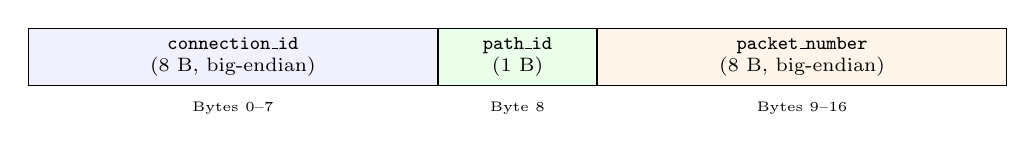
\begin{tikzpicture}[cell/.style={draw, rectangle, minimum height=0.72cm, align=center, font=\scriptsize}, node distance=0cm]
    \node[cell, minimum width=5.2cm, fill=blue!6] (cid) {\code{connection\_id}\\(8 B, big-endian)};
    \node[cell, minimum width=2.0cm, right=of cid, fill=green!8] (pid) {\code{path\_id}\\(1 B)};
    \node[cell, minimum width=5.2cm, right=of pid, fill=orange!8] (pn) {\code{packet\_number}\\(8 B, big-endian)};
    \node[below=0.08cm of cid.south, font=\tiny] {Bytes 0--7};
    \node[below=0.08cm of pid.south, font=\tiny] {Byte 8};
    \node[below=0.08cm of pn.south, font=\tiny] {Bytes 9--16};
\end{tikzpicture}
\caption{Exact 17-byte binary layout of \code{PacketHeader}.}
\label{fig:hdr_layout}
\end{figure}

\begin{table}[H]
\centering
\scriptsize
\begin{tabularx}{\textwidth}{p{2.2cm}cccp{4.4cm}X}
\toprule
\textbf{Field Name} & \textbf{Size (B)} & \textbf{Offset} & \textbf{Role} & \textbf{Purpose} & \textbf{Meaning \& Implementation Notes} \\
\midrule
\code{connection\_id} & 8 & 0 & Transmission & Logical session identifier & Big-endian \code{uint64\_t}. Random 64-bit value on \code{Client}; used by \code{Server::peek\_header()} to route datagrams. \\
\code{path\_id} & 1 & 8 & Transmission / Reliability & Identifies path and PN space & \code{0} for initial path; odd IDs (\code{1, 3, ...}) for client-opened secondary paths. \\
\code{packet\_number} & 8 & 9 & Reliability / ACK & Per-path transmission sequence & Big-endian \code{uint64\_t}, starting at \code{1} per path, strictly monotonic. Never \code{0}. \\
\bottomrule
\end{tabularx}
\caption{Packet header field specification verified against \code{include/packet/packet.hpp} and \code{src/packet/packet.cpp}.}
\label{tab:pkt_header}
\end{table}

\subsection{Frame Formats and Complete Field Breakdown}
Starting at byte 17, right after the header, a packet carries one or more self-delimiting frames (\code{Packet::deserialize()} rejects packets with zero frames). Table~\ref{tab:frame_fields} lists every field of all seven implemented frame types.

\begin{table}[H]
\centering
\scriptsize
\begin{tabularx}{\textwidth}{L{2.2cm}L{2.1cm}ccL{2.28cm}Y}
\toprule
\textbf{Frame (Type Byte)} & \textbf{Field} & \textbf{Size (B)} & \textbf{Offset} & \textbf{Role} & \textbf{Purpose / Meaning} \\
\midrule
\code{STREAM} (\code{0x01}) & \code{type} & 1 & 0 & Transmission & Identifies \code{FRAME\_STREAM} (\code{0x01}); retransmittable. \\
(Header: 16 B) & \code{stream\_id} & 4 & 1 & Transmission & Big-endian \code{uint32\_t} stream identifier (client uses 1, 3, 5\dots). \\
 & \code{offset} & 8 & 5 & Reliability & Big-endian \code{uint64\_t} byte offset within stream. \\
 & \code{fin} & 1 & 13 & Reliability & \code{0} or \code{1}; \code{1} marks end-of-stream at \code{offset + length}. \\
 & \code{length} & 2 & 14 & Transmission & Big-endian \code{uint16\_t} payload length (\code{0} valid only if \code{fin == 1}). \\
 & \code{data} & $L$ & 16 & Payload & Application stream bytes ($0 \le L \le 1317$ in standard packets). \\
\midrule
\code{ACK} (\code{0x02}) & \code{type} & 1 & 0 & Acknowledgement & Identifies \code{FRAME\_ACK} (\code{0x02}); \emph{not} retransmittable. \\
(Header: 16 B + & \code{path\_id} & 1 & 1 & Acknowledgement & Path whose packet-number space is being acknowledged. \\
varint ranges) & \code{largest\_acked} & 8 & 2 & Ack / RTT & Highest packet number observed on \code{path\_id}. \\
 & \code{ack\_delay\_us} & 4 & 10 & RTT & Microseconds receiver held \code{largest\_acked} before sending ACK. \\
 & \code{num\_ranges} & 2 & 14 & Acknowledgement & Count of ACK ranges ($1 \le \text{num\_ranges} \le 256$). \\
 & \code{first\_range\_len} & 1--8 & 16 & Acknowledgement & Varint: $\text{ranges}[0].\text{last} - \text{ranges}[0].\text{first}$ (packets minus 1). \\
 & \code{gap\_i, len\_i} & 2--16 & var. & Acknowledgement & For $i \ge 1$: missing packet count ($\text{prev.first} - r.\text{last} - 1 \ge 1$) and $r.\text{last} - r.\text{first}$. \\
\midrule
\code{CONN\_CLOSE} (\code{0x03}) & \code{type} & 1 & 0 & Transmission & Identifies \code{FRAME\_CONNECTION\_CLOSE}; retransmittable flag true, though sent directly on all paths without tracking. \\
(Header: 7 B) & \code{error\_code} & 4 & 1 & Transmission & \code{0} (\code{NO\_ERROR}), \code{1} (\code{PROTOCOL\_ERROR}), \code{2} (\code{IDLE\_TIMEOUT}). \\
 & \code{reason\_length} & 2 & 5 & Transmission & Reason string length ($\le \text{MAX\_CLOSE\_REASON\_LENGTH} = 200$). \\
 & \code{reason} & $0..200$ & 7 & Transmission & UTF-8/ASCII diagnostic string. \\
\midrule
\code{WINDOW\_UPDATE} & \code{type} & 1 & 0 & Flow Control & Identifies \code{FRAME\_WINDOW\_UPDATE} (\code{0x04}); retransmittable. \\
(\code{0x04}, 13 B) & \code{stream\_id} & 4 & 1 & Flow Control & Target stream ID (\code{0} = connection-level window). \\
 & \code{byte\_offset} & 8 & 5 & Flow Control & New absolute receive window limit in bytes. \\
\midrule
\code{PING} (\code{0x07}, 1 B) & \code{type} & 1 & 0 & Reliability & Single-byte liveness/RTT probe; retransmittable (triggers ACK). \\
\midrule
\code{ADD\_ADDRESS} (\code{0x10}) & \code{type}, \code{num\_addr} & 2 & 0--1 & Transmission & Type (\code{0x10}) and address count ($1 \le N \le 255$); retransmittable. \\
(2 B + $6N$ B) & \code{ipv4}, \code{port} & 4 + 2 & $2+6i$ & Transmission & Raw 4-byte IPv4 (\code{in\_addr}) + big-endian 2-byte UDP port per entry. \\
\midrule
\code{PATHS} (\code{0x12}) & \code{type}, \code{num\_paths} & 2 & 0--1 & Transmission & Type (\code{0x12}) and path count ($1 \le N \le 255$); retransmittable. \\
(2 B + $5N$ B) & \code{path\_id}, \code{rtt\_us} & 1 + 4 & $2+5i$ & Reliability / Sched. & Path ID + smoothed RTT ($\mu$s), or \code{0xFFFFFFFF} if potentially failed. \\
\bottomrule
\end{tabularx}
\caption{Complete frame specifications verified against \code{include/packet/frame.hpp} and \code{src/packet/frame.cpp}. Offset is relative to the start of the frame.}
\label{tab:frame_fields}
\end{table}

\subsection{Packet Size Limits, Varint Encoding, and Validation}
\begin{itemize}
    \item \textbf{Maximum packet size:} \code{MAX\_PACKET\_SIZE = 1350} bytes (\code{packet.hpp:12}). \code{Packet::serialize()} throws \code{std::length\_error} if \code{size() > 1350}.
    \item \textbf{Variable-length integers (varints):} Used exclusively for ACK range lengths and gaps (\code{src/\hspace{0pt}packet/\hspace{0pt}frame.cpp:78-129}). The two most-significant bits of the first byte encode byte length $L = 2^{\text{prefix}}$: \code{00} $\rightarrow$ 1 B ($< 2^6$), \code{01} $\rightarrow$ 2 B ($< 2^{14}$), \code{10} $\rightarrow$ 4 B ($< 2^{30}$), \code{11} $\rightarrow$ 8 B ($< 2^{62}$). Thus 256 worst-case disjoint 1-packet ranges with small gaps require $16 + 1 + 255 \times 2 = 527$ bytes, fitting easily inside 1350 bytes.
    \item \textbf{Deserialization and validation:} \code{Packet::deserialize()} enforces: (a) \code{length >= 18}; (b) at least one valid frame; (c) exact buffer bounds for every field; (d) \code{STREAM} rejects \code{fin > 1} or \code{data\_len == 0 \&\& fin == 0}; (e) \code{ACK} rejects \code{num\_ranges == 0 || num\_ranges > 256}, ranges reaching packet number 0 (\code{first\_length >= largest\_acked} or \code{above\_first < gap + 2} or \code{range\_length >= r.last}), or \code{gap == 0}; (f) \code{PATHS} and \code{ADD\_ADDRESS} reject count $0$; (g) \code{CONNECTION\_CLOSE} rejects \code{reason\_length > 200}; (h) trailing unparsed bytes or unknown frame types fail parsing.
\end{itemize}

\subsection{Packet Number vs.\ Data Offset}
A foundational principle of QUIC and MP-QUIC Mini is separating \emph{transmission identity} (\code{packet\_number}) from \emph{application byte position} (\code{offset}).
\begin{itemize}
    \item \textbf{Packet Number:} Identifies a specific UDP transmission on a specific \code{path\_id}. It is strictly increasing per path ($1, 2, 3, \dots$) and is \emph{never} reused, even for retransmissions. This eliminates the TCP retransmission ambiguity problem: the sender always knows whether an ACK came from the original transmission or a retransmission, ensuring clean RTT samples.
    \item \textbf{Data Offset:} Identifies the logical byte position inside a \code{SendStream}/\code{ReceiveStream} (starting at $0$). It depends only on the stream data, never on which packet or path carries it.
\end{itemize}
\textbf{Worked Retransmission Example:} Suppose Path 0 sends Packet Number \code{5} carrying \code{STREAM(stream\_id=1, offset=2634, length=1317)}. Packet 5 is lost. When \code{SentPacketHandler} detects the loss, it places the \code{STREAM} frame into \code{Connection::retransmission\_queue}. Suppose Path 0 is now marked potentially failed, so \code{LowestRttScheduler} selects Path 1 (whose next packet number is \code{12}), and Path 1 already needs to include a 20-byte \code{ACK} frame. Then \code{add\_retransmission\_frames()} calculates remaining space $1350 - 17 - 20 = 1313$ bytes, leaving $1313 - 16 = 1297$ bytes for stream data. It transmits Packet Number \code{12} on Path 1 containing \code{STREAM(stream\_id=1, offset=2634, fin=0, length=1297)}, and leaves the remaining 20 bytes at \code{offset=3931} in \code{retransmission\_queue} for the next packet (e.g., Path 1 Packet Number \code{13}). At the receiver, \code{StreamFrameSorter} reassembles both slices seamlessly at bytes \code{[2634, 3951)}.

% ==============================================================================
\section{MTU, MSS, and Packet Sizing}
% ==============================================================================

\subsection{Protocol Overhead Layers and Capacity Equations}
In an IPv4 Ethernet network, the link-layer Maximum Transmission Unit (MTU) bounds the largest IP packet that can be transmitted without IP fragmentation:
\begin{itemize}
    \item \textbf{Ethernet MTU:} $1500\text{ bytes}$ (excluding the 14-byte Ethernet header and 4-byte FCS).
    \item \textbf{IPv4 Header:} $20\text{ bytes}$ (standard header without IP options).
    \item \textbf{UDP Header:} $8\text{ bytes}$.
    \item \textbf{UDP Payload Capacity:}
    \begin{equation}
        \text{UDP Payload Capacity} = \text{IP MTU} - \text{IPv4 Header} - \text{UDP Header} = 1500 - 20 - 8 = 1472\text{ bytes}
    \end{equation}
    \item \textbf{TCP MSS vs.\ MP-QUIC Mini Application Payload Capacity:} Standard TCP over IPv4/Ethernet has a Maximum Segment Size of $\text{MSS} = 1500 - 20 - 20 = 1460\text{ bytes}$. In MP-QUIC Mini, each UDP datagram is further capped at \code{MAX\_PACKET\_SIZE = 1350} bytes, with a 17-byte public header and at least a 16-byte \code{STREAM} frame header:
    \begin{equation}
        \text{Max App Payload} = \text{MAX\_PACKET\_SIZE} - \text{HEADER\_SIZE} - \text{STREAM\_FRAME\_HEADER\_SIZE}
    \end{equation}
\end{itemize}

\subsection{Worked Example Using Actual Project Configuration}
Using the exact constants in \code{include/packet/packet.hpp} and \code{include/packet/frame.hpp}:
\begin{align*}
    \text{Max UDP Datagram Payload Sent} &= \text{MAX\_PACKET\_SIZE} = 1350\text{ bytes} \\
    \text{Total IPv4 Packet Size on Wire} &= 1350 + 8\text{ (UDP)} + 20\text{ (IPv4)} = 1378\text{ bytes} < 1500\text{ bytes} \\
    \text{Available Frame Space} &= 1350 - 17\text{ (\code{PacketHeader})} = 1333\text{ bytes} \\
    \text{Max Application Data (single \code{STREAM} frame)} &= 1333 - 16\text{ (\code{STREAM} header)} = 1317\text{ bytes}
\end{align*}
Thus, with no piggybacked ACK or control frames, every full data packet carries $1317$ application bytes, yielding a framing efficiency of $1317 / 1378 \approx 95.6\%$ over IPv4. The $122$-byte margin below the $1472$-byte Ethernet UDP capacity ensures zero IP fragmentation even if a link carries VLAN, PPPoE, or VPN tunneling overhead.

\subsection{Distinction Between Configured Sizes and Congestion MSS}
A subtle implementation detail exists in \code{include/congestion\_control/congestion.hpp:9}:
\begin{itemize}
    \item \textbf{Wire packet cap:} \code{MAX\_PACKET\_SIZE = 1350} bytes governs \code{Packet::serialize()} and \code{Connection} framing.
    \item \textbf{Congestion-window MSS constant:} \code{DEFAULT\_TCP\_MSS = 1460} bytes is used by \code{OliaSender} and \code{FixedWindowCongestion} to convert packet-unit congestion windows into bytes (\code{cwnd\_packets * 1460}). Meanwhile, \code{SentPacketHandler} accumulates \code{bytes\_in\_flight} using actual serialized packet lengths ($\le 1350$ bytes) and tests \code{bytes\_in\_flight > congestion->get\_congestion\_window()}. Consequently, a window of $W$ packets actually allows $\lfloor W \times 1460 / 1350 \rfloor + 1$ full 1350-byte packets in flight.
\end{itemize}

\subsection{Path MTU Support and Limitations}
MP-QUIC Mini does \textbf{not} implement Path MTU Discovery (PMTUD / DPLPMTUD), per-path MTU tracking, or runtime CLI configuration of \code{MAX\_PACKET\_SIZE}. All paths share the compile-time constant \code{MAX\_PACKET\_SIZE = 1350} bytes. If an intermediate link has an MTU smaller than $1378$ bytes, IPv4 fragmentation (or drops if DF is set by the OS/network) will occur transparently beneath UDP.

% ==============================================================================
\section{Connection Management}
% ==============================================================================

\subsection{Logical Connections Over Connectionless UDP}
Although UDP maintains no connection state in the kernel, MP-QUIC Mini establishes stateful logical sessions in user space keyed by a 64-bit \code{connection\_id}. Every packet carries \code{connection\_id} at bytes 0--7. A \code{Client} generates a random 64-bit ID via \code{std::random\_device} (or accepts an explicit ID for tests). A \code{Server} maintains a map \code{std::map<uint64\_t, ServerConnection>} mapping each active \code{connection\_id} to its \code{Connection} and \code{PathManager}, independent of source IP/port changes.

\subsection{Connection Creation, Implicit Setup, and Multi-Path Binding}
There is \textbf{no cryptographic or 3-way handshake}:
\begin{enumerate}
    \item \textbf{Client initiation:} \code{Client::add\_local\_address(ip)} binds one non-blocking \code{UDPSocket} per local interface (default ephemeral port 0, 4~MiB socket buffers). \code{Client::connect(server\_ip, server\_port)} creates \textbf{Path 0} on the first local interface. The first application packet sent on Path 0 opens the connection.
    \item \textbf{Server acceptance:} When \code{Server::handle\_datagram()} receives a packet for an unknown \code{connection\_id} (not in \code{recently\_closed}), it verifies \code{path\_id == 0} and \code{Packet::deserialize()}. It creates a \code{Connection}, configures \code{idle\_timeout\_us}, creates Path 0 via \code{PathManager}, calls \code{connection->advertise\_addresses(get\_listen\_addresses())} to queue an \code{ADD\_ADDRESS} frame, and invokes \code{new\_connection\_callback}.
    \item \textbf{Secondary path creation:} Upon receiving \code{ADD\_ADDRESS}, the client's \code{PathManager::on\_add\_address()} pairs each unused local interface with an unused advertised server address (or falls back to \code{initial\_remote} for single-homed servers), assigns odd Path IDs (\code{1, 3, 5, \dots}), and immediately sends a \code{PING} on each new path. When the server receives a packet with a valid odd \code{path\_id}, \code{PathManager::on\_packet\_received()} dynamically creates that \code{Path} on the server.
    \item \textbf{NAT rebinding:} If a packet arrives on a known \code{path\_id} from a different source IP/port, \code{PathManager::on\_packet\_received()} updates the path's remote address while preserving its packet numbers, RTT, and congestion state.
\end{enumerate}

\subsection{Connection States, Termination, and Error Handling}
Figure~\ref{fig:conn_states} depicts the implemented connection lifecycle. Internally, \code{Connection} tracks boolean flags \code{closed} and \code{closed\_by\_peer}, plus \code{close\_reason}.

\begin{figure}[H]
\centering
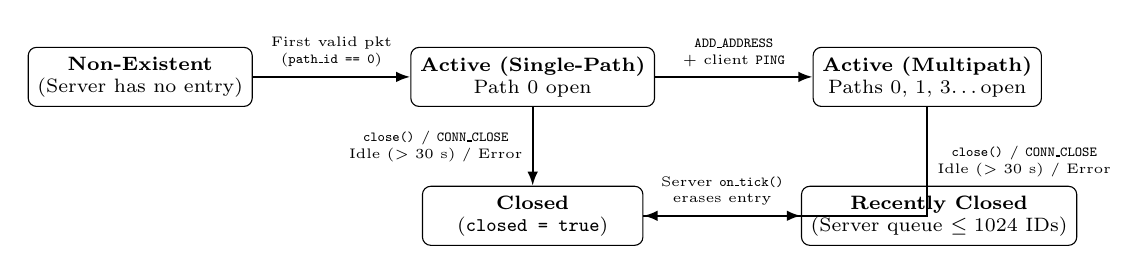
\begin{tikzpicture}[
    state/.style={draw, rectangle, rounded corners=3pt, minimum height=0.75cm, minimum width=2.8cm, align=center, font=\scriptsize},
    arr/.style={-{Latex[length=1.8mm]}, thick}
]
    \node[state] (none) {\textbf{Non-Existent}\\(Server has no entry)};
    \node[state, right=2.0cm of none] (active1) {\textbf{Active (Single-Path)}\\Path 0 open};
    \node[state, right=2.0cm of active1] (active2) {\textbf{Active (Multipath)}\\Paths 0, 1, 3\dots open};
    \node[state, below=1.0cm of active1] (closed) {\textbf{Closed}\\(\code{closed = true})};
    \node[state, right=2.0cm of closed] (recent) {\textbf{Recently Closed}\\(Server queue $\le 1024$ IDs)};

    \draw[arr] (none) -- node[above, font=\tiny, align=center] {First valid pkt\\(\code{path\_id == 0})} (active1);
    \draw[arr] (active1) -- node[above, font=\tiny, align=center] {\code{ADD\_ADDRESS}\\+ client \code{PING}} (active2);
    \draw[arr] (active1) -- node[left, font=\tiny, align=center] {\code{close()} / \code{CONN\_CLOSE}\\Idle ($>30$ s) / Error} (closed);
    \draw[arr] (active2) |- node[near start, right, font=\tiny, align=center] {\code{close()} / \code{CONN\_CLOSE}\\Idle ($>30$ s) / Error} (closed);
    \draw[arr] (closed) -- node[above, font=\tiny, align=center] {Server \code{on\_tick()}\\erases entry} (recent);
\end{tikzpicture}
\caption{Connection state machine implemented across \code{Connection} and \code{Server}.}
\label{fig:conn_states}
\end{figure}

\begin{itemize}
    \item \textbf{Stream FIN vs.\ Connection Close:} Closing a stream (\code{close\_stream(id)}) sets \code{FIN} on the last \code{STREAM} frame of that stream only; the connection remains open for other streams (used by \code{mpq\_reqres} on streams $1, 3, 5, \dots$). Calling \code{Connection::close(reason)} flushes pending ACKs via \code{send\_pending()}, sends a \code{CONNECTION\_CLOSE} frame (\code{CLOSE\_NO\_ERROR = 0}) on \emph{every} path (so a broken path does not prevent delivery), and sets \code{closed = true}.
    \item \textbf{Protocol errors and idle timeout:} Receiving an ACK for an unsent packet or exceeding the receive flow-control window invokes \code{close\_with\_error()} with \code{CLOSE\_PROTOCOL\_ERROR = 1}. Silence exceeding \code{idle\_timeout\_us} (default $30\text{ s}$) triggers \code{close\_with\_error("idle timeout")} with \code{CLOSE\_IDLE\_TIMEOUT = 2}.
    \item \textbf{Late packet suppression:} On the server, \code{on\_tick()} moves closed connection IDs into \code{recently\_closed} (capped at \code{MAX\_RECENTLY\_CLOSED = 1024}) so stray late packets do not resurrect a finished session.
\end{itemize}

% ==============================================================================
\section{Reliability Mechanism}
% ==============================================================================

\subsection{Sender-Side Operations}
\begin{itemize}
    \item \textbf{Segmentation (\code{SendStream}):} Application bytes are stored in a per-stream FIFO queue. During packet construction, \code{pop\_stream\_frame()} removes up to $\min(\text{available\_space} - 16, \text{send\_window\_size})$ bytes and constructs a \code{STREAM} frame stamped with \code{next\_offset}. If the stream was closed and the frame drains the remaining buffer, \code{fin = true} is set.
    \item \textbf{Per-path numbering \& tracking:} Each \code{Path} assigns monotonically increasing packet numbers ($1, 2, 3, \dots$). When \code{Connection::send\_packet()} transmits a packet containing at least one retransmittable frame (any frame other than \code{ACK}), \code{SentPacketHandler::sent\_packet()} inserts a \code{SentPacket} record (storing packet number, retransmittable frames only, serialized length, and timestamp) into \code{packet\_history} (\code{std::map<uint64\_t, SentPacket>}) and adds \code{length} to \code{bytes\_in\_flight}.
    \item \textbf{ACK processing \& loss queuing:} When an ACK arrives, \code{SentPacketHandler::received\_ack()} identifies newly acknowledged packets in \code{packet\_history}, subtracts their lengths from \code{bytes\_in\_flight}, erases them from \code{packet\_history}, resets \code{rto\_count} and \code{tlp\_count}, and triggers time-based loss detection (\code{detect\_lost\_packets()}). Lost packets are moved from \code{packet\_history} to \code{SentPacketHandler::retransmission\_queue}.
    \item \textbf{Cross-path retransmission:} \code{Connection::\hspace{0pt}collect\_retransmissions()} drains every path's queue and pushes \code{STREAM} frames into the connection-wide \code{retransmission\_queue}. Thus, lost stream data is completely decoupled from its original packet and path and is retransmitted on whichever healthy path the scheduler selects next, under a fresh packet number.
\end{itemize}

\subsection{Receiver-Side Operations}
\begin{itemize}
    \item \textbf{Packet reception \& duplicate detection:} \code{ReceivedPacketHandler::is\_duplicate(pn)} checks whether \code{pn} lies inside any stored interval in \code{ranges}. Even for duplicate packets, \code{received\_packet()} records the reception and may trigger an ACK (in case the previous ACK was lost), while \code{Connection::handle\_packet()} skips re-executing the duplicate packet's frames.
    \item \textbf{Reorder buffer (\code{StreamFrameSorter}):} Maintains non-overlapping byte chunks indexed by start offset in \code{std::map<uint64\_t, vector<uint8\_t>> chunks}, along with \code{read\_position} (next undelivered byte offset) and \code{buffered\_bytes}.
    \item \textbf{Overlapping \& duplicate byte trimming:} In \code{StreamFrameSorter::push(offset, data)}, any prefix below \code{read\_position} is clipped. It then inspects existing chunks overlapping $[start, end)$ using \code{chunks.upper\_bound(cur)} and inserts \emph{only} the missing sub-intervals falling in gaps between existing chunks.
    \item \textbf{FIN \& in-order delivery (\code{ReceiveStream}):} Because retransmitted \code{STREAM} frames might be trimmed when overlapping already-buffered data, \code{ReceiveStream} stores \code{fin\_offset = frame.offset + frame.data.size()} separately rather than attaching \code{fin} to a chunk. \code{ReceiveStream::pop()} pops contiguous chunks starting at \code{read\_position} and sets \code{fin = true} exactly when \code{sorter.get\_read\_position() == fin\_offset}.
\end{itemize}

\subsection{Practical Out-of-Order \& Loss Recovery Examples}
\textbf{Out-of-Order Arrival Example (Packets 1 $\rightarrow$ 3 $\rightarrow$ 4 $\rightarrow$ 2):}
Suppose stream 1 sends 4 packets of 1000 bytes each: P1 (offset 0--999), P2 (1000--1999), P3 (2000--2999), P4 (3000--3999) across two paths with different delays, arriving in order $1 \rightarrow 3 \rightarrow 4 \rightarrow 2$:
\begin{enumerate}
    \item \textbf{P1 arrives:} \code{ReceivedPacketHandler} queues immediate ACK (first packet). \code{StreamFrameSorter} stores \code{[0, 1000)}; \code{pop()} matches \code{read\_position == 0}, delivers bytes 0--999 to app, advances \code{read\_position = 1000}.
    \item \textbf{P3 arrives:} \code{ReceivedPacketHandler} records range \code{[3, 3]} alongside \code{[1, 1]} (or across paths if on another path) and queues immediate ACK on detecting a hole. \code{Sorter} stores \code{[2000, 3000)}; \code{pop()} stops because \code{chunks.begin()->first = 2000 != 1000}.
    \item \textbf{P4 arrives:} \code{ReceivedPacketHandler} merges \code{[3, 4]}. \code{Sorter} stores \code{[3000, 4000)}; \code{read\_position} stays $1000$ (\code{buffered\_bytes = 2000}).
    \item \textbf{P2 arrives:} \code{ReceivedPacketHandler} merges \code{[1, 4]} and queues immediate ACK (packet below \code{last\_ack\_largest\_acked}). \code{Sorter} stores \code{[1000, 2000)}. Now \code{pop()} loops three times, delivering \code{[1000, 2000)}, \code{[2000, 3000)}, and \code{[3000, 4000)} strictly in sequence, advancing \code{read\_position = 4000} and \code{buffered\_bytes = 0}.
\end{enumerate}

\textbf{Packet-Loss and Cross-Path Recovery Example:}
If P2 (sent on Path 0 at $t_0$) is dropped in the network while P3 and P4 arrive on Path 0, the receiver sends an ACK with ranges \code{[3,4]} and \code{[1,1]}. On Path 0, \code{SentPacketHandler} checks \code{time\_since\_sent} for P2 against $\frac{9}{8}\text{RTT}$. Once exceeded (either immediately or when the \code{loss\_time} alarm fires), P2 is removed from \code{packet\_history}, \code{bytes\_in\_flight} decreases, \code{OliaSender::on\_packet\_lost()} halves Path 0's \code{cwnd}, and P2's \code{STREAM} frame (offset 1000) moves to \code{Connection::retransmission\_queue}. If Path 1 currently has a lower SRTT or available \code{cwnd}, \code{LowestRttScheduler} schedules the retransmission onto Path 1 under Path 1's next packet number (e.g., PN 7) with the identical stream offset \code{1000}. When PN 7 reaches the receiver, \code{Sorter} fills the \code{[1000, 2000)} hole and delivers bytes 1000--3999 in order.

% ==============================================================================
\section{ACK and SACK Mechanisms}
% ==============================================================================

\subsection{Cumulative vs.\ Selective Acknowledgements and Path Decoupling}
MP-QUIC Mini does not send byte-level cumulative ACKs like TCP. Instead, \code{AckFrame} implements \textbf{packet-number-level Selective Acknowledgements (SACK)} scoped to a specific path:
\begin{itemize}
    \item \code{AckFrame::path\_id} specifies \emph{which} path's packet-number space is being acknowledged.
    \item \code{AckFrame::ranges} stores non-overlapping contiguous intervals $[first, last]$ sorted in \textbf{descending} order ($\text{ranges}[0].\text{last} == \text{largest\_acked}$). When no packets are missing, \code{ranges} has a single range $[1, \text{largest\_acked}]$ (acting as a cumulative ACK). When holes exist, up to \code{MAX\_ACK\_RANGES = 256} disjoint ranges are carried in one \code{ACK} frame.
    \item \textbf{Cross-path ACK delivery:} While \code{Connection::send\_acks\_and\_control\_frames()} sends pure ACKs on the path where the data arrived, an ACK frame generated for Path 0 can also be parsed inside a packet arriving on Path 1 (for example, if a future scheduler or test routes it there). \code{Connection::handle\_frame()} looks up \code{acked\_path = get\_path(frame.ack.path\_id)}. When the ACK arrives on a \emph{different} path (\code{frame.ack.path\_id != packet.get\_path\_id()}), it passes \code{with\_packet\_number = 0} to \code{SentPacketHandler::received\_ack()} because packet numbers from different paths are incomparable.
\end{itemize}

\subsection{Range Maintenance and ACK Generation Triggers}
\code{ReceivedPacketHandler} maintains received packet numbers in \code{std::map<uint64\_t, uint64\_t> ranges} (key = \code{first}, value = \code{last}). When a new packet arrives, \code{add\_to\_history()} either extends an adjacent lower range, extends an adjacent upper range, merges both ranges if it bridges a 1-packet hole, or inserts a singleton $[pn, pn]$. If \code{ranges.size() > 256}, the lowest (oldest) range is erased and \code{lower\_limit} advances to its \code{last} value so dropped old packet numbers are not re-inserted later.

An ACK is queued (\code{ack\_queued = true}, canceling \code{ack\_alarm}) or delayed according to five rules in \code{maybe\_queue\_ack()}:
\begin{enumerate}
    \item \textbf{First packet:} If \code{!has\_last\_ack}, queue ACK immediately.
    \item \textbf{Gap filling:} If \code{packet\_number < last\_ack\_largest\_acked}, queue ACK immediately to notify the sender that a previously missing packet arrived.
    \item \textbf{New hole detected:} If \code{ranges.rbegin()->first > last\_ack\_largest\_acked}, a gap opened above the previous ACK; queue ACK immediately.
    \item \textbf{Every 2nd data packet:} If \code{should\_instigate\_ack} is true (packet contained a non-ACK frame) and \code{retransmittable\_packets\_received\_since\_last\_ack >= 2}, queue ACK immediately.
    \item \textbf{Delayed ACK timer:} Otherwise, if \code{should\_instigate\_ack} is true and \code{ack\_alarm == 0}, arm \code{ack\_alarm = now\_us + 25000} (25~ms). ACK-only packets (\code{should\_instigate\_ack == false}) never trigger an ACK.
\end{enumerate}

\subsection{Impact on Retransmission, RTT, and Congestion Control}
When \code{SentPacketHandler::received\_ack()} accepts an ACK: (1) it filters out reordered ACKs on the same path (\code{with\_packet\_number <= largest\_received\_packet\_with\_ack}) and non-advancing ACKs (\code{ack.largest\_acked <= largest\_in\_order\_acked()}); (2) if \code{ack.largest\_acked} is still in \code{packet\_history}, it feeds \code{rcv\_time\_us - send\_time\_us} and \code{ack.ack\_delay\_us} to \code{RttStats::update\_rtt()}, which may trigger \code{HybridSlowStart} exit; (3) for each newly ACKed packet in \code{determine\_newly\_acked\_packets()}, it removes the packet from \code{packet\_history}, decrements \code{bytes\_in\_flight}, resets \code{rto\_count = tlp\_count = 0}, and invokes \code{OliaSender::on\_packet\_acked()}; (4) it invokes \code{detect\_lost\_packets()} to declare older missing packets below \code{largest\_acked} lost.

% ==============================================================================
\section{Loss Detection, Fast Retransmit, and RTO}
% ==============================================================================

\subsection{Time-Based Loss Detection vs.\ Packet-Threshold Fast Retransmit}
In single-path TCP, receiving 3 duplicate ACKs triggers Fast Retransmit. In multipath transport—or even single-path UDP over multi-queue links—packets frequently experience reordering across paths or queues, causing packet-threshold schemes (such as 3-dupACK) to misinterpret reordering as loss and spuriously halve \code{cwnd}.

Consequently, MP-QUIC Mini does \textbf{not} implement a packet-threshold (dupACK count) Fast Retransmit trigger. Instead, \code{SentPacketHandler::detect\_lost\_packets()} implements \textbf{purely time-based loss detection} (modeled on QUIC loss detection):
\begin{equation}
    \text{delay\_until\_lost} = \left(1 + \frac{1}{8}\right) \cdot \max(\text{latest\_rtt}, \text{smoothed\_rtt}) = \frac{9}{8} \cdot \text{max\_rtt}
\end{equation}
For every unacknowledged packet in \code{packet\_history} with $\text{packet\_number} \le \text{largest\_acked}$:
\begin{itemize}
    \item If $\text{now\_us} - \text{send\_time\_us} > \text{delay\_until\_lost}$, the packet is declared lost: \code{losses++}, it is moved to \code{retransmission\_queue}, and \code{OliaSender::on\_packet\_lost()} is called.
    \item Otherwise, \code{loss\_time} is set to $\text{now\_us} + \text{delay\_until\_lost} - \text{time\_since\_sent}$ for the earliest unacknowledged packet below \code{largest\_acked}, so \code{on\_alarm()} will declare it lost if it remains unacknowledged after $\frac{9}{8}\text{RTT}$.
\end{itemize}
Packets with $\text{packet\_number} > \text{largest\_acked}$ are never judged by \code{detect\_lost\_packets()} (no later ACK has proven reordering/loss); they are covered by Tail Loss Probes and RTO.

\subsection{Tail Loss Probes (TLP) and Retransmission Timeout (RTO)}
When no packet above an unacknowledged packet has been acknowledged (\code{loss\_time == 0}), \code{SentPacketHandler::\hspace{0pt}update\_loss\_detection\_alarm()} arms either a \textbf{Tail Loss Probe} or an \textbf{RTO}:
\begin{itemize}
    \item \textbf{Tail Loss Probe (TLP):} Armed when $\text{smoothed\_rtt} \neq 0$ and $\text{tlp\_count} < \text{MAX\_TAIL\_LOSS\_PROBES} = 2$:
    \begin{equation}
        \text{TLP timeout} =
        \begin{cases}
            \max\!\left(2 \cdot \text{SRTT},\; \frac{3}{2}\cdot\text{SRTT} + \frac{\text{MIN\_RETRANS\_TIME}}{2}\right) & \text{if } |\text{packet\_history}| > 1 \\
            \max\!\left(2 \cdot \text{SRTT},\; \text{MIN\_TLP\_TIMEOUT}\right) & \text{if } |\text{packet\_history}| = 1
        \end{cases}
    \end{equation}
    where $\text{MIN\_RETRANS\_TIME} = 200\text{ ms}$ and $\text{MIN\_TLP\_TIMEOUT} = 10\text{ ms}$. When TLP fires, \code{retransmit\_tlp()} moves the \emph{newest} packet in \code{packet\_history} to \code{retransmission\_queue} and increments \code{tlp\_count}. Crucially, a TLP does \textbf{not} increment \code{losses} and does \textbf{not} notify \code{OliaSender} of loss—it merely provokes an ACK to drive time-based loss detection or confirm path liveness.
    \item \textbf{Retransmission Timeout (RTO):} Armed when no RTT sample exists yet or $\text{tlp\_count} \ge 2$:
    \begin{equation}
        \text{RTO} = \min\!\left(\max\!\left(\text{RTO}_{\text{base}},\, 200\text{ ms}\right) \cdot 2^{\min(\text{rto\_count},\, 16)},\; 60\text{ s}\right)
    \end{equation}
    where $\text{RTO}_{\text{base}} = \text{SRTT} + 4 \cdot \text{mean\_deviation}$ (or $\text{DEFAULT\_RTO\_TIMEOUT\_US} = 500\text{ ms}$ if $\text{SRTT} == 0$), and the alarm is set to $\text{last\_sent\_time} + \max(\text{RTO}, 200\text{ ms})$.
\end{itemize}

\subsection{RTO Path-Failure Handling and Loss Recovery State Machine}
When the RTO alarm expires in \code{SentPacketHandler::on\_alarm(now\_us)}, it invokes \code{Path::on\_rto(last\_sent\_time\_us)}, which checks whether \code{last\_network\_activity\_time < last\_sent\_time\_us}:
\begin{itemize}
    \item \textbf{If false (activity seen since last sent packet):} \code{retransmit\_oldest\_two\_packets()} queues up to the 2 oldest packets as losses, calls \code{OliaSender::on\_retransmission\_timeout(true)}, and updates \code{last\_sent\_time = now\_us} (a custom improvement noted in comments so that a newly broken path will fail on the next RTO rather than trickling 2 packets forever).
    \item \textbf{If true (no activity since last sent packet):} The path is marked \code{potentially\_failed = true}. \code{retransmit\_all\_packets()} dumps \emph{all} remaining packets in \code{packet\_history} into \code{retransmission\_queue} (so \code{Connection} immediately reroutes them onto healthy paths!), calls \code{on\_retransmission\_timeout(true)}, and \code{Connection::on\_tick()} emits a \code{PATHS} frame notifying the peer.
\end{itemize}
Note that MP-QUIC Mini does \textbf{not} enforce a maximum retransmission count; retransmission and exponential-backoff RTO probing continue until data is acknowledged or the 30-second connection idle timeout expires. Figure~\ref{fig:loss_fsm} shows the loss-recovery alarm state machine.

\begin{figure}[H]
\centering
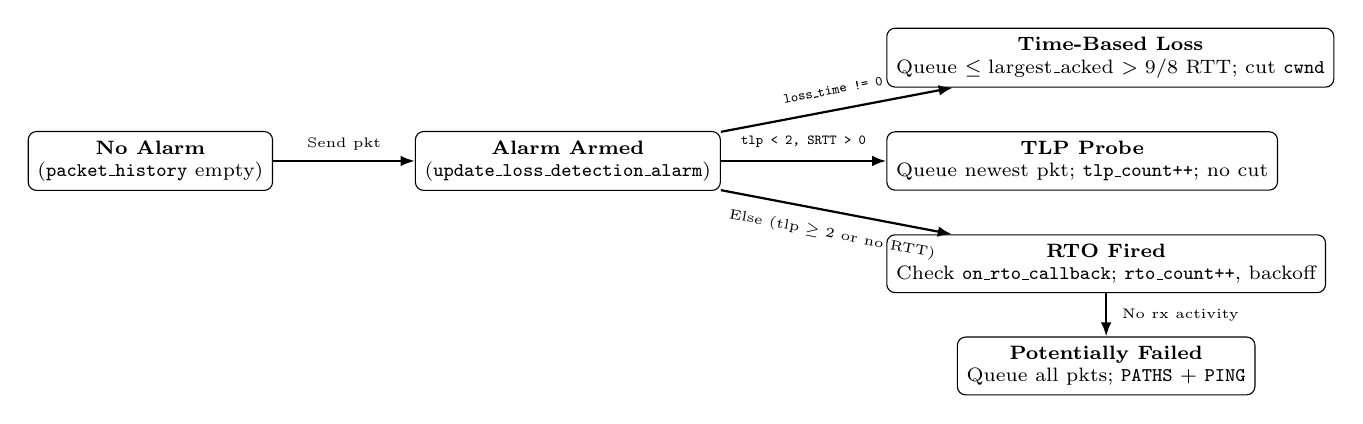
\begin{tikzpicture}[
    st/.style={draw, rectangle, rounded corners=3pt, minimum height=0.72cm, minimum width=2.8cm, align=center, font=\scriptsize},
    arr/.style={-{Latex[length=1.8mm]}, thick}
]
    \node[st] (idle) {\textbf{No Alarm}\\(\code{packet\_history} empty)};
    \node[st, right=1.8cm of idle] (arm) {\textbf{Alarm Armed}\\(\code{update\_loss\_detection\_alarm})};
    \node[st, above right=0.55cm and 2.1cm of arm] (tloss) {\textbf{Time-Based Loss}\\Queue $\le\text{largest\_acked}$ $>9/8\text{ RTT}$; cut \code{cwnd}};
    \node[st, right=2.1cm of arm] (tlp) {\textbf{TLP Probe}\\Queue newest pkt; \code{tlp\_count++}; no cut};
    \node[st, below right=0.55cm and 2.1cm of arm] (rto) {\textbf{RTO Fired}\\Check \code{on\_rto\_callback}; \code{rto\_count++}, backoff};
    \node[st, below=0.55cm of rto] (pf) {\textbf{Potentially Failed}\\Queue all pkts; \code{PATHS} + \code{PING}};

    \draw[arr] (idle) -- node[above, font=\tiny] {Send pkt} (arm);
    \draw[arr] (arm) -- node[above=2pt, sloped, font=\tiny] {\code{loss\_time != 0}} (tloss);
    \draw[arr] (arm) -- node[above=1pt, font=\tiny] {\code{tlp < 2, SRTT > 0}} (tlp);
    \draw[arr] (arm) -- node[below=2pt, sloped, font=\tiny] {Else ($\text{tlp}\ge 2$ or no RTT)} (rto);
    \draw[arr] (rto) -- node[right=2pt, font=\tiny] {No rx activity} (pf);
\end{tikzpicture}
\caption{Sender loss-recovery state machine in \code{SentPacketHandler}.}
\label{fig:loss_fsm}
\end{figure}

% ==============================================================================
\section{RTT Measurement and Timers}
% ==============================================================================

\subsection{Per-Path RTT Estimation Equations}
Each \code{Path} owns an independent \code{RttStats} instance because heterogeneous paths (e.g., 20~ms Wi-Fi vs.\ 50~ms cellular) exhibit distinct latencies and jitter. Mixing RTTs across paths would corrupt both RTO bounds and Lowest-RTT scheduling decisions. All timestamps use \code{std::chrono::steady\_clock} in microseconds (\code{Packet::current\_time\_us()}).

When an ACK acknowledges a packet number matching \code{largest\_acked} that is still in \code{packet\_history}, \code{RttStats::update\_rtt(send\_delta\_us, ack\_delay\_us)} computes (ignoring zero deltas):
\begin{align}
    \text{min\_rtt} &\leftarrow \min(\text{min\_rtt}, \text{send\_delta\_us}) \quad \text{(uncorrected raw RTT)} \\
    \text{sample} &=
    \begin{cases}
        \text{send\_delta\_us} - \text{ack\_delay\_us} & \text{if } \text{send\_delta\_us} > \text{ack\_delay\_us} \\
        \text{send\_delta\_us} & \text{otherwise}
    \end{cases} \\
    \text{latest\_rtt} &\leftarrow \text{sample}
\end{align}
On the first sample ($\text{smoothed\_rtt} == 0$):
\begin{equation}
    \text{SRTT} \leftarrow \text{sample}, \qquad \text{RTTVAR} \ (\text{mean\_deviation}) \leftarrow \frac{\text{sample}}{2}
\end{equation}
On subsequent samples (integer arithmetic, updating deviation first using the prior SRTT):
\begin{align}
    \text{RTTVAR} &\leftarrow \frac{3 \cdot \text{RTTVAR} + |\text{SRTT} - \text{sample}|}{4} \\
    \text{SRTT} &\leftarrow \frac{7 \cdot \text{SRTT} + \text{sample}}{8}
\end{align}
Note that \code{ack\_delay\_us} is computed by the receiver as $\text{now\_us} - \text{largest\_observed\_received\_time}$ (capped at \code{UINT32\_MAX}), preventing the 25~ms delayed-ACK hold time from inflating path RTT estimates.

\subsection{Timer Granularity and Management}
MP-QUIC Mini uses a polling-based timer architecture rather than kernel \code{timerfd} descriptors:
\begin{itemize}
    \item \textbf{Timer resolution:} \code{SocketManager::run(tick\_ms)} wakes from \code{epoll\_wait()} every \code{tick\_ms} ms (default $10\text{ ms}$; configured to $1\text{ ms}$ in \code{mpq\_server}, \code{mpq\_client}, and \code{mpq\_reqres} for fine timer precision).
    \item \textbf{Loss/TLP/RTO alarms:} Checked for every path in \code{Connection::on\_tick()} via \code{sent\_handler->get\_alarm\_timeout() <= now\_us}.
    \item \textbf{Delayed ACK timer:} Checked inside \code{ReceivedPacketHandler::get\_ack\_frame(now\_us, out\_ack)} whenever \code{send\_pending()} runs (on packet arrival and every tick).
    \item \textbf{Idle timer:} Checked at the top of \code{Connection::on\_tick()} against \code{last\_activity\_us + idle\_timeout\_us} (default $30\text{ s}$).
\end{itemize}

% ==============================================================================
\section{Flow Control}
% ==============================================================================

\subsection{Dual-Level Flow Control and Auto-Tuning}
Flow control protects the receiver from buffer exhaustion by limiting how many bytes the sender may transmit ahead of what the receiver's application has consumed. MP-QUIC Mini implements QUIC-style two-level flow control in \code{FlowController} and \code{FlowControlManager}:
\begin{itemize}
    \item \textbf{Stream level (\code{stream\_id} $> 0$):} Initial window $32\text{ KiB}$ ($32768\text{ B}$), auto-tuning ceiling $16\text{ MiB}$. Bounds any single stream from monopolizing receiver memory.
    \item \textbf{Connection level (\code{stream\_id} $= 0$):} Initial window $48\text{ KiB}$ ($49152\text{ B}$), auto-tuning ceiling $24\text{ MiB}$, scaled by \code{CONNECTION\_FLOW\_CONTROL\_MULTIPLIER = 1.5}. Bounds aggregate memory across all streams.
\end{itemize}

\textbf{Receiver Tracking:}
As \code{STREAM} frames arrive, \code{FlowControlManager::update\_highest\_received(stream\_id, frame.offset + data.size())} tracks the highest byte offset seen per stream and adds the incremental growth to the connection-level \code{highest\_received}. If either exceeds its \code{receive\_window}, \code{check\_flow\_control\_violation()} triggers \code{close\_with\_error()}. Notice that because \code{bytes\_read} only increments in \code{handle\_stream\_frame()} after \code{ReceiveStream::pop()} delivers in-order data, any out-of-order data held in \code{StreamFrameSorter} consumes receive-window credit until gaps fill.

\textbf{Window Updates and Auto-Tuning:}
On every \code{send\_pending()}, \code{maybe\_update\_window()} checks whether remaining advertised credit $\text{receive\_window} - \text{bytes\_read}$ has dropped below $\text{receive\_window\_increment} / 2$. If so:
\begin{enumerate}
    \item If $\text{now\_us} - \text{last\_window\_update\_time} < 2 \cdot \max_p(\text{SRTT}_p)$ (and both are non-zero), the window is too small for the connection's bandwidth-delay product, so \code{receive\_window\_increment} is doubled (up to the 16~MiB / 24~MiB cap). When a stream's increment grows, the connection controller's minimum increment is raised via \code{ensure\_minimum\_window\_increment(1.5 * new\_increment)}.
    \item \code{receive\_window} advances to $\text{bytes\_read} + \text{receive\_window\_increment}$, and a \code{WINDOW\_UPDATE} frame is queued on \textbf{all active paths} so loss on one path cannot stall the sender.
\end{enumerate}

\textbf{Sender Enforcement and Resumption:}
Before emitting new stream data, \code{Connection::\hspace{0pt}add\_new\_stream\_frames()} queries \code{send\_window\_size(stream\_id)} $= \min(\text{stream.send\_window} - \text{stream.bytes\_sent},\;\allowbreak \text{conn.send\_window} - \text{conn.bytes\_sent})$. When zero, new stream data (including FIN) stops—though retransmissions and duplicated startup packets do not consume flow-control credit. Sending resumes automatically when a \code{WINDOW\_UPDATE} frame raises \code{send\_window} via \code{update\_send\_window()}.

\subsection{Flow Control vs.\ Congestion Control and Absent Features}
Flow control protects \emph{receiver memory} (end-to-end window between peer endpoints), whereas congestion control protects \emph{network router queues} (per-path bytes in flight). Notably, MP-QUIC Mini does \textbf{not} implement QUIC's \code{BLOCKED} / \code{STREAM\_BLOCKED} frames, dynamic stream-count limits (\code{MAX\_STREAMS}), or handshake-negotiated initial windows (both peers hardcode $32\text{ KiB} / 48\text{ KiB}$).

% ==============================================================================
\section{Congestion Control}
% ==============================================================================

\subsection{Per-Path Controller Architecture and Hybrid Slow-Start}
MP-QUIC Mini defines an abstract \code{CongestionController} interface implemented by \code{FixedWindowCongestion} (a constant-window test stub) and \code{OliaSender} (attached to each \code{Path}). All window accounting in \code{OliaSender} uses packet counts converted to bytes via $\text{cwnd\_bytes} = \text{cwnd\_packets} \times \text{DEFAULT\_TCP\_MSS}$ ($1460\text{ B}$), bounded by $\text{min\_cwnd} = 2\text{ packets}$ and $\text{max\_cwnd} = 2500\text{ packets}$.

\textbf{Slow Start and HyStart:}
Initially, $\text{cwnd} = 32\text{ packets}$ and $\text{ssthresh} = 2500\text{ packets}$. While $\text{cwnd} < \text{ssthresh}$ (Slow Start), each ACK acknowledging a packet when \code{is\_cwnd\_limited()} is true increments \code{cwnd} by $+1$ packet (doubling \code{cwnd} every RTT). Here \code{is\_cwnd\_limited(bytes\_in\_flight)} returns true if $\text{bytes\_in\_flight} \ge \text{cwnd\_bytes}$, or during slow start if $\text{bytes\_in\_flight} > \text{cwnd\_bytes} / 2$, or if remaining window $\le \text{MAX\_BURST\_BYTES} = 3 \times 1460 = 4380\text{ B}$.

To exit slow start before bufferbloat induces packet drops, \code{HybridSlowStart} monitors the first \code{HYBRID\_START\_MIN\_SAMPLES} $= 8$ RTT samples in each packet burst round. At the 8th sample, if $\text{cwnd} \ge$ \code{HYBRID\_START\_LOW\_WINDOW} $= 16$ and the round's minimum RTT exceeds the path's baseline \code{min\_rtt} by a delay threshold:
\begin{equation}
    \text{threshold} = \min\!\left(\max\!\left(\frac{\text{min\_rtt}}{2^3},\; 4000\;\mu\text{s}\right),\; 16000\;\mu\text{s}\right)
\end{equation}
then \code{exit\_slow\_start()} sets $\text{ssthresh} = \text{cwnd}$, transitioning immediately into Congestion Avoidance.

\subsection{Coupled Multipath Congestion Avoidance: OLIA}
Once $\text{cwnd} \ge \text{ssthresh}$, independent TCP-like AIMD across $N$ paths would make one multipath flow $N\times$ more aggressive than a single TCP flow at a shared bottleneck. \code{Connection::add\_path()} links every path's \code{OliaSender} into a shared table \code{olia\_senders} so each path executes the \textbf{Opportunistic Linked-Increases Algorithm (OLIA)} during Congestion Avoidance.

For every ACK on path $r$ (when not in recovery and when \code{is\_cwnd\_limited} is true), path $r$'s window $w_r$ (in packets) increases by:
\begin{equation}
    \Delta w_r = \frac{\dfrac{w_r}{\text{rtt}_r^2}}{\left(\displaystyle\sum_{p \in P} \dfrac{w_p}{\text{rtt}_p}\right)^2} + \frac{\epsilon_r}{w_r}
    \label{eq:olia}
\end{equation}
The first term couples window growth across all paths $P$ so aggregate aggressiveness stays TCP-friendly; the second term shifts capacity from congested largest-window paths to better-performing paths. Let $M = \{p \in P : w_p = \max_q w_q\}$ be the set of paths with the maximum window, and let $B = \arg\max_{p \in P} \frac{l_p}{\text{rtt}_p^2}$ be the set of "best" paths maximizing smoothed bytes acknowledged between losses $l_p = \max(\text{loss}_3 - \text{loss}_2,\; \text{loss}_2 - \text{loss}_1)$ divided by $\text{rtt}_p^2$. Then:
\begin{equation}
    \epsilon_r =
    \begin{cases}
        +\dfrac{1}{|P| \cdot |B \setminus M|} & \text{if } r \in B \setminus M \\[6pt]
        -\dfrac{1}{|P| \cdot |M|} & \text{if } r \in M \text{ and } B \setminus M \neq \emptyset \\[6pt]
        0 & \text{otherwise}
    \end{cases}
\end{equation}

\textbf{128-Bit Fixed-Point Implementation:}
In \code{OliaSender::congestion\_window\_after\_ack()}, \code{OLIA\_SCALE = 10} ($S = 1024$) scales fractional packet increments into integer accumulator \code{snd\_cwnd\_cnt}, using \code{unsigned \_\_int128} (\code{uint128}) to prevent 64-bit overflow when path RTTs differ by orders of magnitude. Letting $\text{rate} = \left(1 + \sum_p w_p S \cdot \frac{\text{rtt}_r}{\text{rtt}_p}\right)^2$, $W = w_r S$, and $\epsilon_r = \frac{\epsilon_{\text{num}}}{\epsilon_{\text{den}}}$, each ACK adds $\frac{S(\epsilon_{\text{num}}\cdot \text{rate} + \epsilon_{\text{den}}\cdot W^2)}{\epsilon_{\text{den}} \cdot w_r \cdot \text{rate}}$ to \code{snd\_cwnd\_cnt}. Whenever \code{snd\_cwnd\_cnt} $\ge 1023$, $w_r \leftarrow w_r + 1$ (and if $\le -1023$ due to negative $\epsilon_r$, $w_r \leftarrow \max(1, w_r - 1)$), resetting \code{snd\_cwnd\_cnt = 0}.

\subsection{Worked Numerical Example of OLIA}
Consider two paths with $\text{rtt}_0 = 20\text{ ms}$, $\text{rtt}_1 = 100\text{ ms}$, and current windows $w_0 = w_1 = 16\text{ packets}$ in Congestion Avoidance:
\begin{itemize}
    \item Suppose both paths have identical bytes-between-losses, or $w_0 = w_1$ so $B \setminus M = \emptyset$; then $\epsilon_0 = \epsilon_1 = 0$.
    \item The coupled denominator is $\sum_p \frac{w_p}{\text{rtt}_p} = \frac{16}{0.02} + \frac{16}{0.10} = 800 + 160 = 960\text{ pkts/s}$, so $(\sum_p w_p/\text{rtt}_p)^2 = 921{,}600$.
    \item On fast Path 0: $\Delta w_0 = \frac{16 / 0.02^2}{921{,}600} = \frac{40{,}000}{921{,}600} \approx 0.0434\text{ packets/ACK}$ ($\approx 23$ ACKs per $+1$ packet).
    \item On slow Path 1: $\Delta w_1 = \frac{16 / 0.10^2}{921{,}600} = \frac{1{,}600}{921{,}600} \approx 0.00174\text{ packets/ACK}$ ($\approx 576$ ACKs per $+1$ packet).
    \item Now suppose Path 0 has $w_0 = 10$ (best path, high bytes between losses) and Path 1 has $w_1 = 20$ (max window, poorer quality) with equal RTTs ($50\text{ ms}$). Then $|P|=2, |B\setminus M|=1, |M|=1$, giving $\epsilon_0 = +1/2$ and $\epsilon_1 = -1/2$. Path 0 gains $\frac{10}{30^2} + \frac{0.5}{10} \approx 0.0611\text{ pkts/ACK}$ (growing in $\sim 17$ ACKs), while Path 1 experiences $\frac{20}{30^2} - \frac{0.5}{20} \approx -0.0028\text{ pkts/ACK}$, smoothly shifting capacity toward Path 0 without packet loss.
\end{itemize}

\subsection{Loss Response, RTO Reset, and Window Comparison}
On packet loss (\code{on\_packet\_lost}), if $\text{packet\_number} > \text{largest\_sent\_at\_last\_cutback}$:
\begin{equation}
    w_r \leftarrow \max\!\left(2,\; \left\lfloor\frac{w_r}{2}\right\rfloor\right), \quad \text{ssthresh}_r \leftarrow w_r, \quad \text{largest\_sent\_at\_last\_cutback} \leftarrow \text{largest\_sent\_packet\_number}
\end{equation}
Only the path that lost the packet cuts its window, and at most once per RTT/burst event; while \code{largest\_acked <= largest\_sent\_at\_last\_cutback} (\code{in\_recovery()}), ACKs do not grow $w_r$. On an RTO (\code{on\_retransmission\_timeout(true)}), \code{SentPacketHandler} first invokes \code{on\_packet\_lost()} (halving $w_r$) and then calls \code{on\_retransmission\_timeout(true)}, which sets $\text{ssthresh}_r \leftarrow w_r / 2$, resets $w_r \leftarrow 2\text{ packets}$, restarts \code{HybridSlowStart}, and clears OLIA's loss-interval history (\code{olia\_reset()}).

Table~\ref{tab:window_terms} distinguishes the four window/size quantities across the codebase.

\begin{table}[H]
\centering
\scriptsize
\begin{tabularx}{\textwidth}{p{2.9cm}p{2.5cm}p{2.2cm}X}
\toprule
\textbf{Term} & \textbf{Scope} & \textbf{Units / Value} & \textbf{Role and Enforcement Location} \\
\midrule
Congestion Window (\code{cwnd}) & Per \code{Path} & Packets ($\times 1460$ B) & Protects network links; \code{SentPacketHandler::sending\_allowed()} blocks new packets when \code{bytes\_in\_flight > cwnd}. \\
Receive Window (\code{send\_window}) & Per stream + Connection & Absolute byte offset & Protects receiver buffers; \code{SendStream::pop\_stream\_frame()} caps new stream bytes via \code{FlowControlManager}. \\
Bytes in Flight & Per \code{Path} & Serialized bytes & Sum of \code{SentPacket::length} in \code{packet\_history} (retransmittable packets awaiting ACK). \\
\code{MAX\_PACKET\_SIZE} / \code{DEFAULT\_TCP\_MSS} & Global constants & $1350\text{ B}$ / $1460\text{ B}$ & $1350\text{ B}$ caps serialized UDP payload; $1460\text{ B}$ converts \code{OliaSender} packet counts to bytes. \\
\bottomrule
\end{tabularx}
\caption{Comparison of congestion window, receive window, bytes in flight, and packet size constants.}
\label{tab:window_terms}
\end{table}

% ==============================================================================
\section{Multipath Scheduling and Path Management}
% ==============================================================================

\subsection{Path Abstraction and Management}
A \code{Path} bundles: (1) an 8-bit \code{path\_id}, (2) local IP/port and remote IP/port, (3) a non-owning pointer to its bound \code{UDPSocket}, (4) an independent 64-bit \code{next\_packet\_number} counter starting at 1, and (5) per-path \code{RttStats}, \code{OliaSender}, \code{SentPacketHandler}, and \code{ReceivedPacketHandler}. Because handlers hold raw pointers to sibling members, \code{Path} is non-copyable.

On the client, \code{PathManager} maintains \code{local\_interfaces}. \code{open\_initial\_path()} creates Path 0 on interface 0; \code{on\_add\_address()} pairs remaining interfaces with server-advertised addresses using odd Path IDs ($1, 3, 5, \dots$) and sends a \code{PING} on each new path so the server discovers it and measures its initial RTT. On the server, \code{PathManager::on\_packet\_received()} accepts only Path 0 and odd Path IDs (rejecting even IDs $> 0$), lazily instantiating \code{Path} objects upon packet arrival and dynamically updating \code{remote\_ip}/\code{remote\_port} on NAT rebinding.

\subsection{Lowest-RTT-First Scheduler (\code{LowestRttScheduler})}
\code{Connection} interacts with \code{Scheduler} (an abstract interface allowing future pluggable schedulers via \code{set\_scheduler()}, though only \code{LowestRttScheduler} is currently implemented). \code{LowestRttScheduler::select\_path(paths, has\_retransmission)} iterates over \code{paths} in ascending \code{path\_id} order and applies these exact rules:
\begin{enumerate}
    \item \textbf{Single-path shortcut:} If $|\text{paths}| == 1$, return that path if \code{has\_retransmission} is true or \code{sending\_allowed()} is true (ignoring \code{potentially\_failed}).
    \item \textbf{All-failed fallback:} If every path is \code{potentially\_failed}, allow all paths to be considered so the connection can recover.
    \item \textbf{CWND filter:} Skip any path where \code{!has\_retransmission \&\& !path->sending\_allowed()}. (Retransmissions bypass CWND checks.)
    \item \textbf{Failure filter:} Skip any \code{potentially\_failed} path (unless all paths failed).
    \item \textbf{RTT selection:} Prefer any path with a known RTT ($\text{SRTT} > 0$) over an unmeasured path ($\text{SRTT} == 0$). Among paths with known RTTs, choose the smallest \code{SRTT} (ties go to the lower \code{path\_id}). If no candidate has a known RTT yet, choose the path with the smallest \code{quota} (packet count sent by the scheduler).
\end{enumerate}

\textbf{Startup Duplication:} If stream data is sent on a path whose \code{SRTT == 0}, \code{Connection::send\_duplicate()} invokes \code{select\_duplicate\_path()}, which returns another non-failed path whose \code{sending\_allowed()} is true and whose \code{quota} is strictly less than the chosen path's \code{quota}. This sends a duplicate copy of the \code{STREAM} frames on the alternate path until an ACK establishes an RTT on the first path.

\textbf{Two-Path Example:} Suppose Path 0 has $\text{SRTT}_0 = 20\text{ ms}$ (Wi-Fi) and Path 1 has $\text{SRTT}_1 = 50\text{ ms}$ (Ethernet/LTE). Initially, both have $\text{SRTT} = 0$: packet 1 goes on Path 0 (\code{quota[0]=1}) and is duplicated onto Path 1 (\code{quota[1]=1}). Once Path 0's ACK returns at $20\text{ ms}$, $\text{SRTT}_0 = 20\text{ ms} > 0$ while $\text{SRTT}_1 = 0$, so all traffic prefers Path 0 until Path 0's CWND fills (\code{sending\_allowed() == false}); traffic then spills onto Path 1, measuring $\text{SRTT}_1 = 50\text{ ms}$. Thereafter, Path 0 is filled first and Path 1 absorbs overflow whenever Path 0's CWND is full.

\subsection{Path Failure Detection, Signaling, and Recovery}
Figure~\ref{fig:path_fsm} illustrates the implemented path health state machine. When Path $p$'s RTO fires and \code{last\_network\_activity\_time < last\_sent\_time\_us}, \code{Path::on\_rto()} marks $p$ as \code{potentially\_failed}. \code{SentPacketHandler} immediately returns all unacknowledged packets on $p$ for cross-path retransmission, \code{Connection::on\_tick()} emits a \code{PATHS} frame (setting $p$'s RTT to \code{0xFFFFFFFF}) on a healthy path so the remote peer also stops sending on $p$, and \code{Connection::collect\_retransmissions()} queues a \code{PING} probe on $p$. Because \code{PING} is retransmittable, its RTO doubles on subsequent timeouts ($200\text{ ms}, 400\text{ ms}, 800\text{ ms}, \dots$ up to $60\text{ s}$), periodically probing $p$ at exponentially decreasing overhead. As soon as \emph{any} valid packet arrives on $p$, \code{Connection::handle\_packet()} clears \code{potentially\_failed = false}, restoring $p$ to active scheduling.

\begin{figure}[H]
\centering
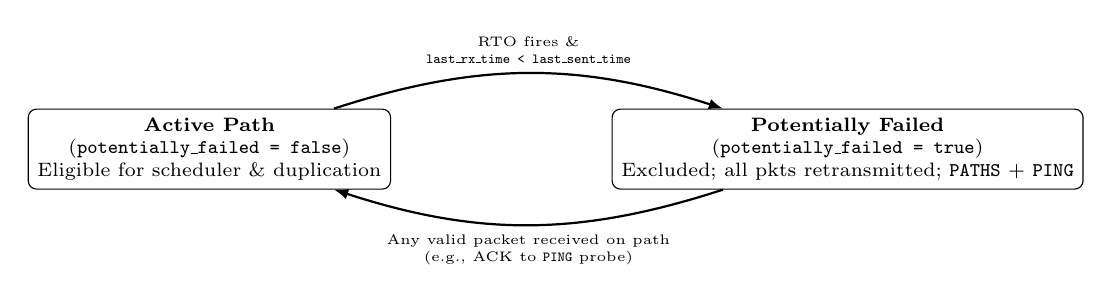
\begin{tikzpicture}[
    st/.style={draw, rectangle, rounded corners=3pt, minimum height=0.8cm, minimum width=3.8cm, align=center, font=\scriptsize},
    arr/.style={-{Latex[length=1.8mm]}, thick}
]
    \node[st] (active) {\textbf{Active Path}\\(\code{potentially\_failed = false})\\Eligible for scheduler \& duplication};
    \node[st, right=2.8cm of active] (failed) {\textbf{Potentially Failed}\\(\code{potentially\_failed = true})\\Excluded; all pkts retransmitted; \code{PATHS} + \code{PING}};

    \draw[arr] (active) to[bend left=18] node[above, font=\tiny, align=center] {RTO fires \&\\ \code{last\_rx\_time < last\_sent\_time}} (failed);
    \draw[arr] (failed) to[bend left=18] node[below, font=\tiny, align=center] {Any valid packet received on path\\(e.g., ACK to \code{PING} probe)} (active);
\end{tikzpicture}
\caption{Implemented path failure and recovery state machine in \code{Path} and \code{Connection}.}
\label{fig:path_fsm}
\end{figure}

% ==============================================================================
\section{Linux Socket Architecture and Event Handling}
% ==============================================================================

\subsection{Non-Blocking UDP Sockets and Kernel Buffers}
Each \code{UDPSocket} opens an IPv4 non-blocking datagram socket via \code{socket(AF\_INET, SOCK\_DGRAM | SOCK\_NONBLOCK, 0)}. Blocking sockets cannot be used safely in a single-threaded multipath loop because a \code{recvfrom()} call on an idle path would stall timer checks and transmission on all other paths. \code{Client::add\_local\_address()} and \code{Server::listen()} invoke \code{UDPSocket::set\_buffer\_size(4 * 1024 * 1024)} to request 4~MiB \code{SO\_RCVBUF} and \code{SO\_SNDBUF} kernel buffers, preventing burst drops during high-rate slow-start or multi-path arrivals.

\subsection{\code{epoll} Event Loop and Syscall Stack Interaction}
\code{SocketManager} creates an epoll instance via \code{epoll\_create1(0)} and registers each socket with \code{EPOLLIN} (level-triggered). In \code{SocketManager::run(tick\_ms)}:
\begin{enumerate}
    \item \code{epoll\_wait(epoll\_fd, events, 16, tick\_ms)} sleeps in the kernel with zero CPU consumption until at least one socket has queued datagrams or \code{tick\_ms} milliseconds elapse. (\code{EINTR} is safely retried.)
    \item For each ready file descriptor, \code{SocketManager} drains all available datagrams in a tight \code{while (true)} loop calling \code{sock->recvFrom(buffer, 65536, src\_ip, src\_port)}, breaking when \code{received <= 0} (which covers \code{EAGAIN}/\code{EWOULDBLOCK} as well as empty reads).
    \item Each datagram triggers the registered \code{RecvCallback} (\code{Client::handle\_datagram} or \code{Server::handle\_datagram}), traversing \code{Connection::handle\_packet()} and sending immediate responses.
    \item After processing ready sockets (or on timeout), \code{tick\_callback()} runs \code{on\_tick()} to advance idle timers, loss-recovery alarms, and pending transmissions.
\end{enumerate}

\begin{figure}[H]
\centering
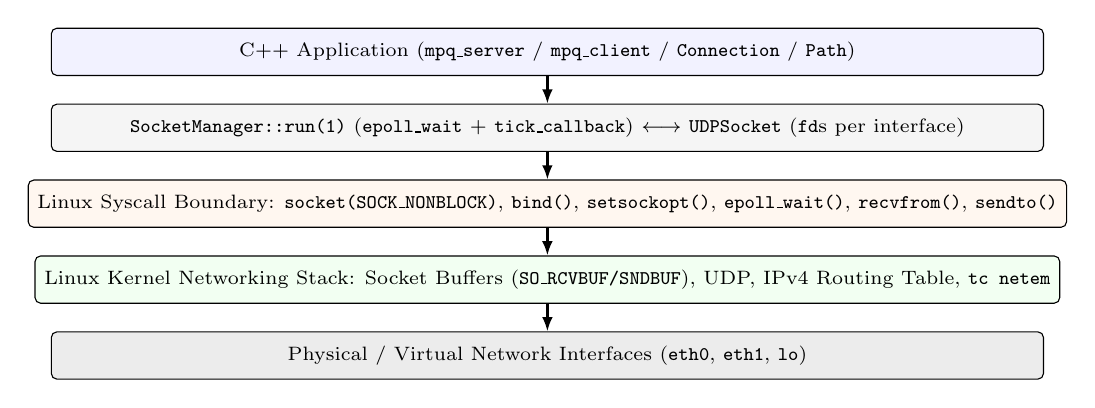
\begin{tikzpicture}[
    box/.style={draw, rectangle, rounded corners=2pt, minimum height=0.6cm, minimum width=12.6cm, align=center, font=\scriptsize},
    arr/.style={-{Latex[length=1.8mm]}, thick}
]
    \node[box, fill=blue!5] (app) {C++ Application (\code{mpq\_server} / \code{mpq\_client} / \code{Connection} / \code{Path})};
    \node[box, below=0.35cm of app, fill=gray!8] (sockmgr) {\code{SocketManager::run(1)} (\code{epoll\_wait} + \code{tick\_callback}) $\longleftrightarrow$ \code{UDPSocket} (\code{fd}s per interface)};
    \node[box, below=0.35cm of sockmgr, fill=orange!6] (posix) {Linux Syscall Boundary: \code{socket(SOCK\_NONBLOCK)}, \code{bind()}, \code{setsockopt()}, \code{epoll\_wait()}, \code{recvfrom()}, \code{sendto()}};
    \node[box, below=0.35cm of posix, fill=green!5] (kern) {Linux Kernel Networking Stack: Socket Buffers (\code{SO\_RCVBUF/SNDBUF}), UDP, IPv4 Routing Table, \code{tc netem}};
    \node[box, below=0.35cm of kern, fill=gray!15] (nic) {Physical / Virtual Network Interfaces (\code{eth0}, \code{eth1}, \code{lo})};

    \draw[arr] (app) -- (sockmgr);
    \draw[arr] (sockmgr) -- (posix);
    \draw[arr] (posix) -- (kern);
    \draw[arr] (kern) -- (nic);
\end{tikzpicture}
\caption{Interaction between MP-QUIC Mini user-space I/O, POSIX syscalls, and the Linux kernel stack.}
\label{fig:linux_io}
\end{figure}

Socket error handling: \code{UDPSocket::sendTo()} and \code{bind()} log errors to \code{stdout} via \code{strerror(errno)} and return \code{-1} or \code{false}. At the protocol layer, a failed \code{sendTo()} is treated identically to a packet lost in transit—it still enters \code{SentPacketHandler} and recovers via loss detection or path failover.

% ==============================================================================
\section{Project Implementation Phases}
% ==============================================================================

The codebase follows a 12-phase incremental architecture documented in \code{README.md} and verified by phase-aligned unit and integration tests. Table~\ref{tab:phases} summarizes every phase against the actual repository state.

\begin{table}[H]
\centering
\scriptsize
\setlength{\tabcolsep}{4pt}
\begin{tabularx}{\textwidth}{L{0.85cm}L{2.65cm}L{3.15cm}YL{2.35cm}L{1.65cm}}
\toprule
\textbf{Phase} & \textbf{Objective \& Problem Solved} & \textbf{Main Classes \& Files} & \textbf{How It Works \& Key Parameters} & \textbf{Tests} & \textbf{Status} \\
\midrule
1 & Non-blocking UDP I/O \& multiplexing without busy-wait & \code{UDPSocket}, \code{SocketManager} (\code{sockets/*}) & \code{SOCK\_NONBLOCK}, \code{epoll\_wait(tick\_ms=10/1)}, 4~MiB buffers & \code{test\_packet\_socket} & Implemented \\
2 & Per-interface path state & \code{Path} (\code{path/path.*}) & Pairs endpoints + \code{UDPSocket*}; monotonic PN space ($\ge 1$) & \code{test\_endpoints} & Implemented \\
3 & Binary wire format & \code{Packet}, \code{Frame} (\code{packet/*}) & 17 B header + 7 frame types; \code{MAX\_PACKET\_SIZE=1350}; varint ACKs & \code{test\_packet} (10 checks) & Implemented \\
4--5 & Stream slicing, RTT \& reliable ACKs & \code{SendStream}, \code{RttStats}, \code{Sent/\hspace{0pt}ReceivedPacketHandler}, \code{Connection} & 16 B \code{STREAM} hdr; 256-range ACKs; 25~ms delayed ACK; EWMA RTT & \code{test\_reliability} (7 checks) & Implemented \\
6--7 & Reassembly, loss recovery, flow control & \code{StreamFrameSorter}, \code{ReceiveStream}, \code{FlowController/Manager} & Overlap trimming; $9/8\text{ RTT}$ loss, 2 TLPs, RTO ($0.2$--$60\text{ s}$); $32\text{ K}/48\text{ K}\to 16\text{ M}/24\text{ M}$ FC & \code{test\_loss\_recovery} (10 checks) & Implemented \\
8 & Multipath scheduling & \code{Scheduler}, \code{LowestRttScheduler} (\code{scheduler/*}) & Lowest-SRTT path selection; startup duplication; \code{PATHS} + \code{PING} probes & \code{test\_scheduler} (6 checks) & Implemented \\
9--10 & Coupled congestion control & \code{OliaSender}, \code{HybridSlowStart}, \code{FixedWindowCongestion} & \code{cwnd} $32$--$2500$ pkts; HyStart ($8$ samples); 128-bit OLIA ($\text{scale}=2^{10}$) & \code{test\_congestion} (10 checks) & Implemented \\
11 & Multi-homed endpoints \& CLI tools & \code{Client}, \code{Server}, \code{PathManager}, \code{mpq\_*}, \code{Sha256} (\code{apps/*}) & Implicit setup on Path 0; \code{ADD\_ADDRESS}; $30\text{ s}$ idle timeout; file/RPC apps & \code{test\_endpoints}, \code{test\_connection}, \code{test\_file\_transfer.sh} & Implemented \\
12 & Real-network evaluation & \code{evaluation/scripts/*.sh} (8 bash scripts) & 4-VM \code{tc netem} topology, \code{iperf3} TCP/UDP/MPTCP baselines, handover & Scripts ready; no VM CSVs recorded & Pending execution \\
\bottomrule
\end{tabularx}
\caption{Phase-by-phase breakdown mapped to actual repository classes, parameters, tests, and status.}
\label{tab:phases}
\end{table}

\textbf{Phase Progression:} Phase~1 establishes raw packet transport; Phase~2 binds sockets to paths; Phase~3 defines the 17-byte container and self-delimiting frames; Phases~4--5 build stream segmentation, per-path packet tracking, SACK generation, and EWMA RTT estimation; Phases~6--7 close the reliability loop with out-of-order reassembly, three-tier loss detection, and dual-level flow control; Phase~8 adds Lowest-RTT scheduling and startup duplication; Phases~9--10 couple path congestion windows via HyStart and OLIA; Phase~11 wraps everything in \code{Client}/\code{Server}/\code{PathManager} and user-facing file/RPC binaries; and Phase~12 provides the multi-VM benchmarking harness.

% ==============================================================================
\section{VM Deployment and Network Topology}
% ==============================================================================

\subsection{Four-VM Evaluation Topology and Documentation Discrepancy}
As implemented in \code{evaluation/scripts/config.sh}, \code{setup\_addresses.sh}, \code{shape\_links.sh}, and \code{README.md}, the evaluation testbed uses \textbf{four Linux machines/VMs} forming two completely disjoint routed paths (matching Figure~3 of the CoNEXT 2017 paper): \textbf{Client}, \textbf{Router A}, \textbf{Router B}, and \textbf{Server}. (Note: \code{PROJECT\_REPORT.tex} in the repository root erroneously depicts a two-VM direct topology; the actual scripts require four machines and \code{shape\_links.sh} exits with an error if executed on Client or Server. Furthermore, no Linux network-namespace scripts exist in the repository.)

\begin{figure}[H]
\centering
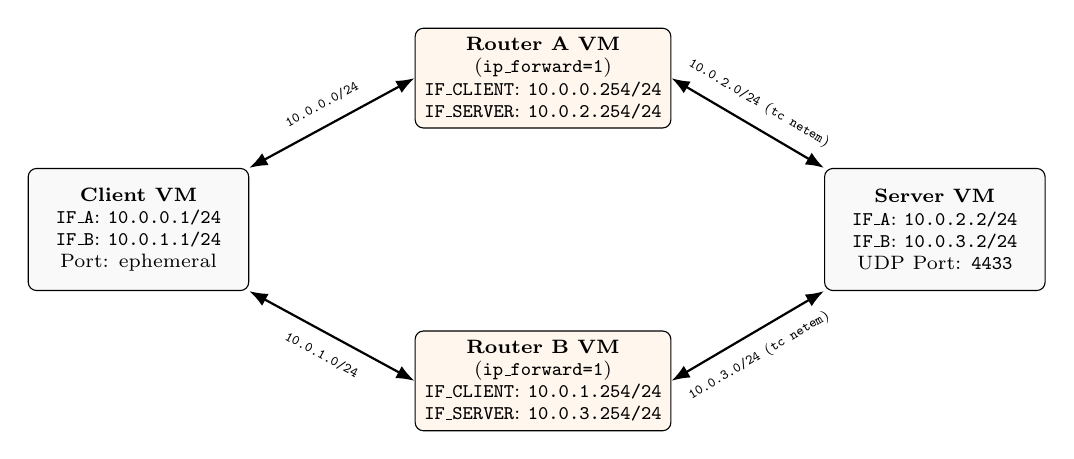
\begin{tikzpicture}[
    nodebox/.style={draw, rectangle, rounded corners=3pt, minimum height=1.55cm, minimum width=2.8cm, align=center, font=\scriptsize, fill=gray!5},
    rbox/.style={draw, rectangle, rounded corners=3pt, minimum height=1.25cm, minimum width=3.2cm, align=center, font=\scriptsize, fill=orange!7},
    arr/.style={Latex-Latex, thick}
]
    \node[nodebox] (cli) {\textbf{Client VM}\\\code{IF\_A}: \code{10.0.0.1/24}\\\code{IF\_B}: \code{10.0.1.1/24}\\Port: ephemeral};
    \node[rbox, above right=0.5cm and 2.1cm of cli] (ra) {\textbf{Router A VM}\\(\code{ip\_forward=1})\\\code{IF\_CLIENT}: \code{10.0.0.254/24}\\\code{IF\_SERVER}: \code{10.0.2.254/24}};
    \node[rbox, below right=0.5cm and 2.1cm of cli] (rb) {\textbf{Router B VM}\\(\code{ip\_forward=1})\\\code{IF\_CLIENT}: \code{10.0.1.254/24}\\\code{IF\_SERVER}: \code{10.0.3.254/24}};
    \node[nodebox, right=7.3cm of cli] (srv) {\textbf{Server VM}\\\code{IF\_A}: \code{10.0.2.2/24}\\\code{IF\_B}: \code{10.0.3.2/24}\\UDP Port: \code{4433}};

    \draw[arr] (cli.north east) -- node[above=2pt, sloped, font=\tiny] {\code{10.0.0.0/24}} (ra.west);
    \draw[arr] (ra.east) -- node[above=2pt, sloped, font=\tiny] {\code{10.0.2.0/24} (\code{tc netem})} (srv.north west);
    \draw[arr] (cli.south east) -- node[below=2pt, sloped, font=\tiny] {\code{10.0.1.0/24}} (rb.west);
    \draw[arr] (rb.east) -- node[below=2pt, sloped, font=\tiny] {\code{10.0.3.0/24} (\code{tc netem})} (srv.south west);
\end{tikzpicture}
\caption{Exact four-VM topology configured by \code{evaluation/scripts/config.sh} and \code{setup\_addresses.sh}.}
\label{fig:4vm}
\end{figure}

\textbf{Routing Behavior:}
On Client, \code{10.0.2.0/24} routes via \code{10.0.0.254} on \code{IF\_A}, and \code{10.0.3.0/24} routes via \code{10.0.1.254} on \code{IF\_B}. Symmetrically, on Server, \code{10.0.0.0/24} routes via \code{10.0.2.254} on \code{IF\_A}, and \code{10.0.1.0/24} routes via \code{10.0.3.254} on \code{IF\_B}. Both routers enable \code{net.ipv4.ip\_forward=1} and apply \code{tc netem} shaping on \emph{both} their \code{IF\_CLIENT} and \code{IF\_SERVER} interfaces so forward and reverse directions experience the configured delay, bandwidth, loss, and queue limit.

\subsection{Reproducible Step-by-Step Deployment Instructions}
\begin{enumerate}
    \item \textbf{VM requirements:} Four Ubuntu Linux VMs (tested scripts reference Ubuntu cloud images; Linux kernel $\ge 5.6$ required only if running optional MPTCP baselines), each with two virtual NICs attached to the corresponding isolated virtual switches/subnets shown in Figure~\ref{fig:4vm}, $\ge 1$ vCPU, and $\ge 1\text{ GiB}$ RAM.
    \item \textbf{Install required packages (Execute on Client, Router A, Router B, Server VMs):}\\
    \code{sudo apt update \&\& sudo apt install -y build-essential g++ make git iproute2 ethtool python3 iperf3 mptcpize}\\
    On Ubuntu cloud images lacking \code{sch\_netem}, also run on \textbf{Router A \& Router B}:\\
    \code{sudo apt install -y linux-modules-extra-\$(uname -r)}
    \item \textbf{Transfer or clone the project (Execute on Host or inside each VM):}\\
    Clone the repository or copy it via \code{scp -r MP\_QUIC user@<vm-ip>:\textasciitilde{}/MP\_QUIC} onto all four VMs, then \code{cd \textasciitilde{}/MP\_QUIC}.
    \item \textbf{Build the project (Execute on Client VM and Server VM):}\\
    \code{make} \quad (Note: the project uses \code{Makefile} with \code{g++ -std=c++17 -Wall -Wextra -O2 -pthread}; there is no \code{CMakeLists.txt}.)
    \item \textbf{Verify interface names (Execute on each VM):}\\
    \code{ip -br link} \quad (Identify the two interface names, e.g., \code{enp0s8} and \code{enp0s9}.)
    \item \textbf{Configure IP addresses, routes, and IP forwarding (Execute on each respective VM):}
    \begin{itemize}
        \item \textbf{Client VM:} \code{./evaluation/scripts/setup\_addresses.sh client <IF\_A> <IF\_B>}
        \item \textbf{Server VM:} \code{./evaluation/scripts/setup\_addresses.sh server <IF\_A> <IF\_B>}
        \item \textbf{Router A VM:} \code{./evaluation/scripts/setup\_addresses.sh router-a <IF\_CLIENT> <IF\_SERVER>}
        \item \textbf{Router B VM:} \code{./evaluation/scripts/setup\_addresses.sh router-b <IF\_CLIENT> <IF\_SERVER>}
    \end{itemize}
    \item \textbf{Verify base connectivity (Execute on Client VM):}\\
    \code{ping -c 2 -I 10.0.0.1 10.0.2.2} \quad and \quad \code{ping -c 2 -I 10.0.1.1 10.0.3.2}
    \item \textbf{Apply network impairments via \code{tc netem} (Execute identically on Router A VM and Router B VM):}\\
    \code{./evaluation/\hspace{0pt}scripts/\hspace{0pt}shape\_links.sh --rate-a 8mbit --delay-a 10ms --loss-a 0}\\
    \code{\ \ --rate-b 4mbit --delay-b 25ms --loss-b 0 --queue 50}\\
    (\code{shape\_links.sh} automatically disables TSO/GSO/GRO via \code{ethtool -K} and detects whether it is on Router A or B. Inspect with \code{./evaluation/scripts/shape\_links.sh show}.)
    \item \textbf{Start the server (Execute on Server VM):}\\
    \code{./evaluation/scripts/start\_server.sh}\\
    This generates \code{evaluation/files/test20M.bin} and \code{test256K.bin} with \code{.sha256} digests, optionally starts \code{iperf3} on ports \code{5201} (TCP/UDP) and \code{5202} (MPTCP), and launches \code{bin/mpq\_server --listen 10.0.2.2:4433 --listen 10.0.3.2:4433 --dir evaluation/files}.
    \item \textbf{Start the client manually or via scripts (Execute on Client VM):}\\
    Manual transfer: \code{./bin/mpq\_client --server 10.0.2.2:4433 --local 10.0.0.1 --local 10.0.1.1 --get test20M.bin --out /tmp/test20M.bin}\\
    Or run the automated suites described in Section~\ref{sec:bench}.
    \item \textbf{Clean up the environment (Execute on Router A, Router B, and Server VMs):}\\
    Stop \code{start\_server.sh} with \code{Ctrl-C} on \textbf{Server VM}; remove shaping on \textbf{Router A \& Router B VMs} with \code{./evaluation/scripts/shape\_links.sh clear}.
\end{enumerate}

% ==============================================================================
\section{Throughput Measurement and Benchmarking}
\label{sec:bench}
% ==============================================================================

\subsection{Metrics, Throughput vs.\ Goodput, and Integrity Verification}
\begin{itemize}
    \item \textbf{Throughput vs.\ Goodput:} \emph{Throughput} measures all bytes crossing the link interface (including 17 B MP-QUIC headers, 16 B frame headers, ACKs, \code{WINDOW\_UPDATE}s, startup duplicates, and retransmissions), captured per-interface via kernel \code{/sys/class/net/<IF>/statistics/rx\_bytes} (\code{rx\_a\_bytes}, \code{rx\_b\_bytes}). \emph{Goodput} measures only useful application payload delivered in order to the client, computed in \code{mpq\_client.cpp:200} as $\text{goodput\_kbps} = \frac{\text{received\_bytes} \times 8}{\text{time\_ms}}$, where \code{time\_ms} spans from first request write to receipt of the stream \code{FIN}.
    \item \textbf{Packet Loss, Retransmissions, RTT:} Reported per path by \code{print\_path\_statistics()} and sampled every $100\text{ ms}$ into CSV when \code{--stats FILE} is passed (\code{StatsWriter}: \code{time\_ms}, \code{path\_id}, \code{packets\_sent}, \code{packets\_lost}, \code{packets\_retransmitted}, \code{packets\_received}, \code{cwnd\_packets}, \code{ssthresh\_packets}, \code{slow\_start}, \code{srtt\_us}, \code{bytes\_in\_flight}, \code{potentially\_failed}, \code{bytes\_transferred}).
    \item \textbf{Handover Recovery Time:} Measured per-request by \code{mpq\_reqres} (default 35 requests of 750~B every 400~ms) in \code{delay\_ms} from request write to response \code{FIN}.
    \item \textbf{CPU Utilization:} Not instrumented by the repository's benchmark scripts (can be measured externally using \code{/usr/bin/time -v} or \code{pidstat}).
    \item \textbf{SHA-256 Integrity:} \code{mpq\_client} computes a streaming FIPS 180-4 SHA-256 digest (\code{apps/sha256.cpp}), and \code{run\_transfers.sh} verifies that both \code{sha256sum} on disk and \code{mpq\_client}'s reported hash match \code{<file>.sha256} downloaded from the server.
    \item \textbf{Experimental Aggregation Benefit ($E_{\text{Ben}}$):} Computed by \code{summary.sh} comparing multipath goodput $G_m$ against single-path goodputs $G_a, G_b$ ($G_{\max} = \max(G_a, G_b)$):
    \begin{equation}
        E_{\text{Ben}} =
        \begin{cases}
            \dfrac{G_m - G_{\max}}{G_a + G_b - G_{\max}} & \text{if } G_m \ge G_{\max} \quad (1 = \text{perfect aggregation}) \\[8pt]
            \dfrac{G_m - G_{\max}}{G_{\max}} & \text{if } G_m < G_{\max} \quad (0 = \text{best single link},\; -1 = \text{zero})
        \end{cases}
    \end{equation}
\end{itemize}

\subsection{Supported Benchmark Commands and Experiments}
All benchmark commands execute on the \textbf{Client VM} while \code{start\_server.sh} runs on the \textbf{Server VM} and \code{shape\_links.sh} sets path conditions on \textbf{Routers A \& B}:
\begin{itemize}
    \item \textbf{Large \& Short File Transfers (Single vs.\ Multipath):}\\
    \code{./evaluation/scripts/run\_transfers.sh --file test20M.bin --runs 3 --label default --stats}\\
    \code{./evaluation/scripts/run\_transfers.sh --file test256K.bin --runs 3 --label short}\\
    Tests \code{multipath\_a\_first}, \code{multipath\_b\_first}, \code{single\_a}, and \code{single\_b}, appending to \code{evaluation/\hspace{0pt}results/\hspace{0pt}throughput.csv}.
    \item \textbf{Baseline Protocol Comparison (UDP, TCP, MPTCP):}\\
    \code{./evaluation/scripts/run\_baselines.sh --bytes 20M --runs 3 --label default}\\
    Runs \code{iperf3} in reverse (\code{-R}) mode for UDP, single-path TCP, and MPTCP (\code{mptcpize run iperf3}).
    \item \textbf{Link Degradation \& Loss Scenarios:} Configure asymmetric RTTs or loss on Routers A \& B via \code{shape\_links.sh --rate-a 20mbit --delay-a 5ms --loss-a 1 --rate-b 2mbit --delay-b 40ms --loss-b 2} and re-run \code{run\_transfers.sh --label lossy}.
    \item \textbf{Network Handover (Link Failure):}\\
    \code{./evaluation/scripts/run\_handover.sh --cut-after 3 --count 35 --label default}\\
    (Also supports \code{--single-path} and \code{--no-cut}.) At $t = 3\text{ s}$, installs \code{tc clsact} egress and ingress \code{matchall action drop} filters on \code{IF\_A} to simulate complete link outage, then reports pre-cut median delay, post-cut median delay, and peak handover latency. Note: \code{run\_handover.sh} does not restore Link A mid-test; path recovery after restoration is instead verified in \code{tests/integration/test\_connection.cpp} (\code{handover} scenario).
    \item \textbf{Aggregation Summary:}\\
    \code{./evaluation/scripts/summary.sh --label default}
\end{itemize}
Note also: only \code{LowestRttScheduler} is implemented; Round-Robin scheduling experiments are not supported without implementing an additional \code{Scheduler} subclass.

\subsection{Verification Observed and Benchmark Results Template}
No Phase~12 VM benchmark CSV files exist in the repository yet (\code{evaluation/results/} is absent and \code{README.md} lists Phase~12 as unchecked). However, running \code{make test} on the local host confirmed all 10 test executables and scripts pass on loopback: \code{test\_packet} (11/11), \code{test\_reliability} (7/7), \code{test\_loss\_recovery} (10/10), \code{test\_scheduler} (6/6), \code{test\_congestion} (10/10), \code{test\_sha256} (2/2), \code{test\_packet\_socket} (1/1), \code{test\_endpoints} (6/6), \code{test\_connection} (11/11 simulated scenarios including 5\% loss, 10\% reordering, $8+4\text{ Mbit/s}$ bottlenecks, and link failure/recovery), and \code{test\_file\_transfer.sh} (7/7 multi-process checks). Table~\ref{tab:bench_template} provides the empty recording template matching \code{summary.sh} output for Phase~12 VM runs.

\begin{table}[H]
\centering
\scriptsize
\setlength{\tabcolsep}{4pt}
\begin{tabularx}{\textwidth}{L{2.05cm}YcccccL{1.25cm}}
\toprule
\textbf{Protocol} & \textbf{Configuration} & \textbf{Runs} & \textbf{Goodput (kbps)} & \textbf{Time (ms)} & \textbf{Link A / B (\%)} & \textbf{$E_{\text{Ben}}$} & \textbf{SHA-256} \\
\midrule
UDP (\code{iperf3}) & \code{single\_a} / \code{single\_b} & -- & \textit{TBD} & \textit{TBD} & 100/0 \;/\; 0/100 & N/A & N/A \\
TCP (\code{iperf3}) & \code{single\_a} / \code{single\_b} & -- & \textit{TBD} & \textit{TBD} & 100/0 \;/\; 0/100 & N/A & N/A \\
MPTCP & \code{multipath\_a\_first} / \code{b\_first} & -- & \textit{TBD} & \textit{TBD} & \textit{TBD} & \textit{TBD} & N/A \\
MP-QUIC Mini & \code{single\_a} / \code{single\_b} & -- & \textit{TBD} & \textit{TBD} & 100/0 \;/\; 0/100 & N/A & Pass/Fail \\
MP-QUIC Mini & \code{multipath\_a\_first} / \code{b\_first} & -- & \textit{TBD} & \textit{TBD} & \textit{TBD} & \textit{TBD} & Pass/Fail \\
\bottomrule
\end{tabularx}
\caption{Phase~12 VM benchmark results template (no VM measurements have been recorded in the repository yet).}
\label{tab:bench_template}
\end{table}

% ==============================================================================
\section{Important Configuration Parameters}
% ==============================================================================

Table~\ref{tab:params} consolidates all protocol, socket, congestion, flow-control, timer, and evaluation parameters verified across the source files.

{\scriptsize
\setlength{\tabcolsep}{4pt}
\begin{longtable}{L{3.15cm}L{1.65cm}L{0.75cm}L{3.05cm}L{1.72cm}L{4.63cm}}
\toprule
\textbf{Parameter} & \textbf{Value} & \textbf{Unit} & \textbf{Source Location} & \textbf{Config.} & \textbf{Purpose \& Effect of Changing} \\
\midrule
\endfirsthead
\toprule
\textbf{Parameter} & \textbf{Value} & \textbf{Unit} & \textbf{Source Location} & \textbf{Config.} & \textbf{Purpose \& Effect of Changing} \\
\midrule
\endhead
\code{HEADER\_SIZE} & 18 & B & \code{packet.hpp:35} & Hardcoded & Fixed public header size; changing alters wire compatibility. \\
\code{MAX\_PACKET\_SIZE} & 1350 & B & \code{packet.hpp:12} & Hardcoded & Max UDP payload; raising near 1472 risks IP fragmentation over tunnels. \\
IP/UDP MTU & 1500 (unspec.) & B & Not in code & OS/Link & Relies on standard 1500 B Ethernet MTU; no PMTUD implemented. \\
Max STREAM payload & 1317 & B & \code{packet.hpp}, \code{frame.hpp} & Derived & $1350 - 17 - 16$; max single-frame app payload per packet. \\
\code{SOCKET\_BUFFER\_SIZE} & 4,194,304 & B & \code{client.cpp:8}, \code{server.cpp:8} & Hardcoded & \code{SO\_RCVBUF}/\code{SO\_SNDBUF} request; prevents burst drops. \\
Number of paths & Dynamic ($\le 128$ client) & paths & \code{path\_manager.hpp:73} & Runtime CLI & Path 0 + odd IDs $1..255$ from \code{--local} args; 1 byte \code{path\_id}. \\
\code{INITIAL\_CONGESTION\_WINDOW} & 32 & pkts & \code{congestion.hpp:10} & Constructor arg & Initial \code{cwnd} per path; higher speeds start-up but risks burst loss. \\
\code{DEFAULT\_MAX\_CONGESTION\_WINDOW} & 2500 & pkts & \code{olia\_sender.hpp:12} & Constructor arg & Upper cap on \code{cwnd}; bounds max BDP per path ($\approx 3.65\text{ MB}$). \\
\code{DEFAULT\_MINIMUM\_CONGESTION\_WINDOW} & 2 & pkts & \code{olia\_sender.hpp:13} & Hardcoded & Floor on \code{cwnd} after loss/RTO; prevents total stall. \\
Initial \code{ssthresh} & 2500 & pkts & \code{olia\_sender.cpp:20} & Hardcoded & Equals \code{max\_cwnd} until HyStart or first packet loss. \\
\code{DEFAULT\_TCP\_MSS} & 1460 & B & \code{congestion.hpp:9} & Hardcoded & Converts \code{cwnd} packets to bytes; diverges slightly from 1350 B max packet. \\
\code{MAX\_TRACKED\_SENT\_PACKETS} & 5000 & pkts & \code{sent\_packet\_handler.hpp:12} & Hardcoded & Max in-flight + queued packets per path ($2\times 2500$); caps memory. \\
\code{MAX\_BURST\_BYTES} & 4380 & B & \code{olia\_sender.hpp:14} & Hardcoded & $3 \times 1460$; allows \code{cwnd} growth when within 3 MSS of full. \\
\code{OLIA\_SCALE} / \code{DIVISOR} & 10 / 2 & bits / -- & \code{olia\_sender.hpp:17,22} & Hardcoded & $2^{10}$ fixed-point precision; loss divides \code{cwnd} by 2. \\
HyStart low window / samples & 16 pkts / 8 & -- & \code{hybrid\_slow\_start.hpp:9,10} & Hardcoded & Min \code{cwnd} and samples/round before HyStart can exit slow start. \\
HyStart delay bounds & $\text{minRTT}/8$, $[4,16]$ & ms & \code{hybrid\_slow\_start.hpp:11-13} & Hardcoded & Queue-delay threshold to exit slow start prior to drop. \\
\code{DEFAULT\_RTO\_TIMEOUT\_US} & 500,000 & $\mu$s & \code{sent\_packet\_handler.hpp:13} & Hardcoded & Initial RTO before first RTT sample. \\
\code{MIN\_RTO} / \code{MAX\_RTO} & 0.2 / 60 & s & \code{sent\_packet\_handler.hpp:14,15} & Hardcoded & Clamps $\text{SRTT}+4\cdot\text{RTTVAR}$ and exponential backoff. \\
\code{MIN\_TLP} / \code{MAX\_TLPS} & 10~ms / 2 & -- & \code{sent\_packet\_handler.hpp:17,18} & Hardcoded & Min TLP interval and probes sent before triggering RTO. \\
Time loss threshold & $9/8\times \text{RTT}$ & -- & \code{sent\_packet\_handler.cpp:184} & Hardcoded & Reordering tolerance before declaring missing packet lost. \\
Fast-retransmit dupACK thr. & N/A & -- & Not implemented & -- & Uses time-based loss ($9/8\text{ RTT}$) instead of dupACK count. \\
Max retransmission count & Uncapped & -- & Not implemented & -- & Retransmits until ACKed or connection \code{idle\_timeout\_us} fires. \\
\code{ACK\_SEND\_DELAY\_US} & 25,000 & $\mu$s & \code{received\_packet\_handler.hpp:10} & Hardcoded & Delayed ACK timer; \code{RETRANSMITTABLE\_PACKETS\_BEFORE\_ACK = 2}. \\
\code{MAX\_ACK\_RANGES} & 256 & ranges & \code{frame.hpp:43} & Hardcoded & Max SACK blocks in one \code{ACK} frame. \\
\code{RECEIVE\_STREAM\_FC\_WIN} & 32 KiB (max 16 MiB) & B & \code{flow\_controller.hpp:11,13} & Hardcoded & Initial/max per-stream receive buffer \& flow-control credit. \\
\code{RECEIVE\_CONN\_FC\_WIN} & 48 KiB (max 24 MiB) & B & \code{flow\_controller.hpp:12,14} & Hardcoded & Initial/max connection receive credit ($1.5\times$ stream multiplier). \\
Scheduler & \code{lowest-rtt} & -- & \code{connection.hpp:156} & API setter & Only \code{LowestRttScheduler} exists; \code{set\_scheduler()} allows swapping. \\
\code{epoll} \code{tick\_ms} & 10 (1 in apps) & ms & \code{socket\_manager.hpp:21} & Runtime arg & Event-loop wake interval; 1~ms gives finer TLP/RTO/ACK timing. \\
\code{DEFAULT\_IDLE\_TIMEOUT\_US} & 30 & s & \code{connection.hpp:22} & CLI \code{--idle-timeout} & Closes silent connections; server tracks \code{1024} \code{recently\_closed} IDs. \\
\code{tc netem} defaults & 8M/10ms, 4M/25ms, q=50 & -- & \code{shape\_links.sh:18-24} & CLI flags & Emulated link rates, one-way delays, 0\% loss, 50-pkt router queue. \\
\bottomrule
\caption{Consolidated reference of all configuration parameters in MP-QUIC Mini.}
\label{tab:params}
\end{longtable}
}

% ==============================================================================
\section{Limitations, Discrepancies, and Future Improvements}
% ==============================================================================

\subsection{Implementation Status Classification}
\begin{itemize}
    \item \textbf{Fully Implemented:} Non-blocking UDP + \code{epoll} reactor; 17-byte public header and 7 self-delimiting frame formats (with 256-range varint ACK codec); per-path packet number spaces, EWMA RTT estimation, time-based loss detection, TLPs, and exponential RTO; out-of-order stream reassembly with overlap trimming; dual-level auto-tuning flow control; Lowest-RTT scheduler with startup duplication, path-failure detection, \code{PATHS} signaling, and \code{PING} recovery; HyStart and 128-bit coupled OLIA congestion control; dynamic \code{PathManager} with NAT rebinding; \code{mpq\_server}, \code{mpq\_client}, \code{mpq\_reqres}, and SHA-256 verification.
    \item \textbf{Partially Implemented:} \code{PATHS} frame transmits per-path SRTTs, but receivers only process the \code{PATHS\_RTT\_POTENTIALLY\_FAILED} sentinel; \code{Scheduler} interface exists for pluggable policies, but only \code{LowestRttScheduler} is implemented; Phase~12 evaluation scripts are complete, but real VM benchmark runs have not been executed/logged.
    \item \textbf{Not Implemented:} TLS 1.3 handshake, payload encryption, and packet-number protection; Path MTU Discovery; \code{CLOSE\_PATH} (\code{0x11}) frame; \code{BLOCKED}/\code{STREAM\_BLOCKED} and \code{MAX\_STREAMS} frames; packet pacing; Round-Robin/BLEST/ECF schedulers; packet-threshold loss detection; maximum retransmission cap; multi-threading; IPv6 support (\code{AF\_INET} only).
\end{itemize}

\subsection{Discrepancies Identified Between Documentation and Code}
\begin{enumerate}
    \item \textbf{VM Topology in \code{PROJECT\_REPORT.tex}:} \code{PROJECT\_REPORT.tex} describes a 2-VM topology and instructs running \code{shape\_links.sh} on Client and Server VMs, whereas \code{evaluation/scripts/} and \code{README.md} implement a 4-VM routed topology where \code{shape\_links.sh} explicitly refuses to run on Client or Server.
    \item \textbf{CWND Byte Scaling vs.\ Wire Packet Cap:} \code{OliaSender} scales packet counts by \code{DEFAULT\_TCP\_MSS = 1460}, whereas \code{Packet::serialize()} caps packets at \code{MAX\_PACKET\_SIZE = 1350}, allowing roughly 8\% more packets in flight than the nominal packet count.
    \item \textbf{Minor Claims in \code{PROJECT\_REPORT.tex}:} \code{SocketManager} breaks on \code{recvFrom() <= 0} without checking \code{EAGAIN}/\code{EWOULDBLOCK}, and \code{LowestRttScheduler} breaks ties by \code{quota} only when RTTs are unknown (equal known RTTs tie-break by lowest \code{path\_id}).
\end{enumerate}

\subsection{Future Improvements}
Key next steps include: (1) executing Phase~12 benchmarks across the 4-VM testbed to collect empirical goodput, $E_{\text{Ben}}$, and handover curves; (2) adding AEAD encryption and a cryptographic handshake (e.g., libsodium/OpenSSL) to prevent spoofing and eavesdropping; (3) implementing \code{CLOSE\_PATH} (\code{0x11}) and alternative schedulers (Round-Robin, BLEST) behind the \code{Scheduler} interface; (4) aligning \code{OliaSender}'s MSS constant with \code{MAX\_PACKET\_SIZE} and adding packet pacing to prevent slow-start micro-bursts; and (5) supporting IPv6 and DPLPMTUD.

% ==============================================================================
\section{Conclusion}
% ==============================================================================

MP-QUIC Mini demonstrates a clean, modular, and verifiable user-space multipath transport protocol built in C++17 over Linux non-blocking UDP sockets and \code{epoll}. By pairing a 17-byte public header with 7 self-delimiting frame types and independent per-path packet number spaces, the implementation cleanly separates transmission tracking from stream-offset ordering. Time-based loss detection ($\frac{9}{8}\text{RTT}$), Tail Loss Probes, and RTO with path-failure signaling prevent cross-path reordering from crippling throughput and allow lost frames to be retransmitted across surviving paths. Coupled 128-bit OLIA congestion control with Hybrid Slow-Start maintains fairness with single-path flows while shifting window capacity to higher-quality paths, and dual-level auto-tuning flow control protects receiver memory across multiple concurrent streams. Together with \code{PathManager}, \code{mpq\_server}, \code{mpq\_client}, \code{mpq\_reqres}, and a passing 10-suite unit and loopback integration harness, the project establishes a solid, inspectable foundation for multi-VM multipath performance evaluation.

\end{document}
